% ******************************* PhD Thesis Template **************************
% Please have a look at the README.md file for info on how to use the template

\documentclass[a4paper,12pt,times,numbered,print,index]{Classes/PhDThesisPSnPDF}

% ******************************************************************************
% ******************************* Class Options ********************************
% *********************** See README for more details **************************
% ******************************************************************************

% `a4paper'(The University of Cambridge PhD thesis guidelines recommends a page
% size a4 - default option) or `a5paper': A5 Paper size is also allowed as per
% the Cambridge University Engineering Deparment guidelines for PhD thesis
%
% `11pt' or `12pt'(default): Font Size 10pt is NOT recommended by the University
% guidelines
%
% `oneside' or `twoside'(default): Printing double side (twoside) or single
% side.
%
% `print': Use `print' for print version with appropriate margins and page
% layout. Leaving the options field blank will activate Online version.
%
% `index': For index at the end of the thesis
%
% `draftclassic': For draft mode without loading any images (same as draft in book)
%
% `draft': Special draft mode with line numbers, images, and water mark with
% timestamp and custom text. Position of the text can also be modified.
%
% `abstract': To generate only the title page and abstract page with
% dissertation title and name, to submit to the Student Registry
%
% `chapter`: This option enables only the specified chapter and it's references
%  Useful for review and corrections.
%
% ************************* Custom Page Margins ********************************
%
% `custommargin`: Use `custommargin' in options to activate custom page margins,
% which can be defined in the preamble.tex. Custom margin will override
% print/online margin setup.
%
% *********************** Choosing the Fonts in Class Options ******************
%
% `times' : Times font with math support. (The Cambridge University guidelines
% recommend using times)
%
% `fourier': Utopia Font with Fourier Math font (Font has to be installed)
%            It's a free font.
%
% `customfont': Use `customfont' option in the document class and load the
% package in the preamble.tex
%
% default or leave empty: `Latin Modern' font will be loaded.
%
% ********************** Choosing the Bibliography style ***********************
%
% `authoryear': For author-year citation eg., Krishna (2013)
%
% `numbered': (Default Option) For numbered and sorted citation e.g., [1,5,2]
%
% `custombib': Define your own bibliography style in the `preamble.tex' file.
%              `\RequirePackage[square, sort, numbers, authoryear]{natbib}'.
%              This can be also used to load biblatex instead of natbib
%              (See Preamble)
%
% **************************** Choosing the Page Style *************************
%
% `default (leave empty)': For Page Numbers in Header (Left Even, Right Odd) and
% Chapter Name in Header (Right Even) and Section Name (Left Odd). Blank Footer.
%
% `PageStyleI': Chapter Name next & Page Number on Even Side (Left Even).
% Section Name & Page Number in Header on Odd Side (Right Odd). Footer is empty.
%
% `PageStyleII': Chapter Name on Even Side (Left Even) in Header. Section Number
% and Section Name in Header on Odd Side (Right Odd). Page numbering in footer

% Uncomment to change page style
%\pagestyle{PageStyleII}

% ********************************** Preamble **********************************
% Preamble: Contains packages and user-defined commands and settings
% ******************************************************************************
% ****************************** Custom Margin *********************************

% Add `custommargin' in the document class options to use this section
% Set {innerside margin / outerside margin / topmargin / bottom margin}  and
% other page dimensions
\ifsetCustomMargin
  \RequirePackage[left=37mm,right=30mm,top=35mm,bottom=30mm]{geometry}
  \setFancyHdr % To apply fancy header after geometry package is loaded
\fi

% Add spaces between paragraphs
%\setlength{\parskip}{0.5em}
% Ragged bottom avoids extra whitespaces between paragraphs
\raggedbottom
% To remove the excess top spacing for enumeration, list and description
%\usepackage{enumitem}
%\setlist[enumerate,itemize,description]{topsep=0em}

% *****************************************************************************
% ******************* Fonts (like different typewriter fonts etc.)*************

% Add `customfont' in the document class option to use this section

\ifsetCustomFont
  % Set your custom font here and use `customfont' in options. Leave empty to
  % load computer modern font (default LaTeX font).
  %\RequirePackage{helvet}

  % For use with XeLaTeX
  %  \setmainfont[
  %    Path              = ./libertine/opentype/,
  %    Extension         = .otf,
  %    UprightFont = LinLibertine_R,
  %    BoldFont = LinLibertine_RZ, % Linux Libertine O Regular Semibold
  %    ItalicFont = LinLibertine_RI,
  %    BoldItalicFont = LinLibertine_RZI, % Linux Libertine O Regular Semibold Italic
  %  ]
  %  {libertine}
  %  % load font from system font
  %  \newfontfamily\libertinesystemfont{Linux Libertine O}
\fi

% *****************************************************************************
% **************************** Custom Packages ********************************

% ************************* Algorithms and Pseudocode **************************

%\usepackage{algpseudocode}


% ********************Captions and Hyperreferencing / URL **********************

% Captions: This makes captions of figures use a boldfaced small font.
%\RequirePackage[small,bf]{caption}

\RequirePackage[labelsep=space,tableposition=top]{caption}
\renewcommand{\figurename}{Fig.} %to support older versions of captions.sty


% *************************** Graphics and figures *****************************

%\usepackage{rotating}
%\usepackage{wrapfig}

% Uncomment the following two lines to force Latex to place the figure.
% Use [H] when including graphics. Note 'H' instead of 'h'
%\usepackage{float}
%\restylefloat{figure}

% Subcaption package is also available in the sty folder you can use that by
% uncommenting the following line
% This is for people stuck with older versions of texlive
%\usepackage{sty/caption/subcaption}
\usepackage{subcaption}

% ********************************** Tables ************************************
\usepackage{booktabs} % For professional looking tables
\usepackage{multirow}

%\usepackage{multicol}
%\usepackage{longtable}
%\usepackage{tabularx}


% *********************************** SI Units *********************************
\usepackage{siunitx} % use this package module for SI units


% ******************************* Line Spacing *********************************

% Choose linespacing as appropriate. Default is one-half line spacing as per the
% University guidelines

% \doublespacing
% \onehalfspacing
% \singlespacing


% ************************ Formatting / Footnote *******************************

% Don't break enumeration (etc.) across pages in an ugly manner (default 10000)
%\clubpenalty=500
%\widowpenalty=500

%\usepackage[perpage]{footmisc} %Range of footnote options


% *****************************************************************************
% *************************** Bibliography  and References ********************

%\usepackage{cleveref} %Referencing without need to explicitly state fig /table

% Add `custombib' in the document class option to use this section
\ifuseCustomBib
   \RequirePackage[square, sort, numbers, authoryear]{natbib} % CustomBib

% If you would like to use biblatex for your reference management, as opposed to the default `natbibpackage` pass the option `custombib` in the document class. Comment out the previous line to make sure you don't load the natbib package. Uncomment the following lines and specify the location of references.bib file

%\RequirePackage[backend=biber, style=numeric-comp, citestyle=numeric, sorting=nty, natbib=true]{biblatex}
%\bibliography{References/references} %Location of references.bib only for biblatex

\fi

% changes the default name `Bibliography` -> `References'
\renewcommand{\bibname}{References}


% ******************************************************************************
% ************************* User Defined Commands ******************************
% ******************************************************************************

% *********** To change the name of Table of Contents / LOF and LOT ************

%\renewcommand{\contentsname}{My Table of Contents}
%\renewcommand{\listfigurename}{My List of Figures}
%\renewcommand{\listtablename}{My List of Tables}


% ********************** TOC depth and numbering depth *************************

\setcounter{secnumdepth}{2}
\setcounter{tocdepth}{2}


% ******************************* Nomenclature *********************************

% To change the name of the Nomenclature section, uncomment the following line

%\renewcommand{\nomname}{Symbols}


% ********************************* Appendix ***********************************

% The default value of both \appendixtocname and \appendixpagename is `Appendices'. These names can all be changed via:

%\renewcommand{\appendixtocname}{List of appendices}
%\renewcommand{\appendixname}{Appndx}

% *********************** Configure Draft Mode **********************************

% Uncomment to disable figures in `draft'
%\setkeys{Gin}{draft=true}  % set draft to false to enable figures in `draft'

% These options are active only during the draft mode
% Default text is "Draft"
%\SetDraftText{DRAFT}

% Default Watermark location is top. Location (top/bottom)
%\SetDraftWMPosition{bottom}

% Draft Version - default is v1.0
%\SetDraftVersion{v1.1}

% Draft Text grayscale value (should be between 0-black and 1-white)
% Default value is 0.75
%\SetDraftGrayScale{0.8}


% ******************************** Todo Notes **********************************
%% Uncomment the following lines to have todonotes.

%\ifsetDraft
%	\usepackage[colorinlistoftodos]{todonotes}
%	\newcommand{\mynote}[1]{\todo[author=kks32,size=\small,inline,color=green!40]{#1}}
%\else
%	\newcommand{\mynote}[1]{}
%	\newcommand{\listoftodos}{}
%\fi

% Example todo: \mynote{Hey! I have a note}


% ************************ Thesis Information & Meta-data **********************
% Thesis title and author information, refernce file for biblatex
% ************************ Thesis Information & Meta-data **********************
%% The title of the thesis
\title{Constructing Hard Examples for Graph Isomorphism}
%\texorpdfstring is used for PDF metadata. Usage:
%\texorpdfstring{LaTeX_Version}{PDF Version (non-latex)} eg.,
%\texorpdfstring{$sigma$}{sigma}

%% Subtitle (Optional)
%% \subtitle{Using the CUED template}

%% The full name of the author
\author{Kashif R. Khan}

%% Department (eg. Department of Engineering, Maths, Physics)
\dept{Computer Laboratory}

%% University and Crest
\university{University of Cambridge}
% Crest minimum should be 30mm.
\crest{
\includegraphics[width=0.2\textwidth]{University_Crest}}
%% Use this crest, if you are using the college crest
%% Crest long miminum should be 65mm
%\crest{
\includegraphics[width=0.45\textwidth]{University_Crest_Long}}

%% College shield [optional] 
% Crest minimum should be 30mm.
%\collegeshield{
\includegraphics[width=0.2\textwidth]{CollegeShields/Kings}}


%% Supervisor (optional)
%% for multiple supervisors, append each supervisor with the \newline command
\supervisor{Prof. Anuj Dawar}

%% Supervisor Role (optional) - Supervisor (default) or advisor
% \supervisorrole{\textbf{Supervisors: }}
%% if no title is desired:
% \supervisorrole{}

%% Supervisor line width: required to align supervisors
%\supervisorlinewidth{0.35\textwidth}

%% Advisor (optional)
%% for multiple advisors, append each advisor with the \newline command
%\advisor{Dr. A. Advisor\newline
%Dr. B. Advisor}
     
%% Advisor Role (optional) - Advisor (default) or leave empty
% \advisorrole{Advisors: }
%% if no title is required
% \advisorrole{}

%% Advisor line width: required to align supervisors
%\advisorlinewidth{0.25\textwidth}


%% You can redefine the submission text:
% Default as per the University guidelines:
% ``This dissertation is submitted for the degree of''
%\renewcommand{\submissiontext}{change the default text here if needed}

%% Full title of the Degree
\degreetitle{Master of Philosophy}

%% College affiliation (optional)
\college{Sidney Sussex College}

%% Submission date
% Default is set as {\monthname[\the\month]\space\the\year}
%\degreedate{September 2014} 

%% Meta information
\subject{LaTeX} \keywords{{LaTeX} {PhD Thesis} {Engineering} {University of
Cambridge}}


% ***************************** Abstract Separate ******************************
% To printout only the titlepage and the abstract with the PhD title and the
% author name for submission to the Student Registry, use the `abstract' option in
% the document class.

\ifdefineAbstract
 \pagestyle{empty}
 \includeonly{Declaration/declaration, Abstract/abstract}
\fi

% ***************************** Chapter Mode ***********************************
% The chapter mode allows user to only print particular chapters with references
% Title, Contents, Frontmatter are disabled by default
% Useful option to review a particular chapter or to send it to supervisior.
% To use choose `chapter' option in the document class

\ifdefineChapter
 \includeonly{Chapter3/chapter3}
\fi

% ******************************** Front Matter ********************************
\begin{document}

\frontmatter

\maketitle

% ******************************* Thesis Dedidcation ********************************

\begin{dedication} 

I would like to dedicate this thesis to my loving parents \dots

\end{dedication}


\newpage
{\Huge \bf Declaration}

\vspace{24pt} 

I \authorname of \authorcollege, being a candidate for the M.Phil in
Advanced Computer Science, hereby declare that this report and the
work described in it are my own work, unaided except as may be
specified below, and that the report does not contain material that
has already been used to any substantial extent for a comparable
purpose.

\vspace{24pt}
Total word count: \wordcount

\vspace{60pt}
\textbf{Signed}: 

\vspace{12pt}
\textbf{Date}:


\vfill

This dissertation is copyright \copyright 2010 \authorname. 
\\
All trademarks used in this dissertation are hereby acknowledged.



\newpage
\vspace*{\fill}

% ************************** Thesis Acknowledgements **************************

\begin{acknowledgements}      

I would like to thank my project supervisor Professor Anuj Dawar for ceaseless support, advice and mentoring throughout this project. I am grateful for his continuous  patience and insight.

I would also like to thank my family, friends and the Computer Laboratory faculty for their kindness and guidance.

\end{acknowledgements}

\newpage
{\Huge \bf Abstract}
\vspace{24pt} 


This is the abstract. Write a summary of the whole thing. Make 
sure it fits in one page. 


\newpage
\vspace*{\fill}


% *********************** Adding TOC and List of Figures ***********************

\tableofcontents

\listoffigures

\listoftables

% \printnomenclature[space] space can be set as 2em between symbol and description
%\printnomenclature[3em]

\printnomenclature

% ******************************** Main Matter *********************************
\mainmatter

%!TEX root = ../thesis.tex
%*******************************************************************************
%*********************************** First Chapter *****************************
%*******************************************************************************
% Andy Pitts
% Haaroon

\chapter{Introduction}  %Title of the First Chapter

\ifpdf
    \graphicspath{{Chapter1/Figs/Raster/}{Chapter1/Figs/PDF/}{Chapter1/Figs/}}
\else
    \graphicspath{{Chapter1/Figs/Vector/}{Chapter1/Figs/}}
\fi
Determining if two graphs $G=(V,E)$ and $G'=(V',E')$ are identical is equivalent to questioning the existence of a bijective function between vertex sets $V$ and $V'$ which preserves edges. If there is such a function $f:V \rightarrow V'$, then we say that the graphs are isomorphic to one another $G{\simeq}G'$ and that there is an isomorphism $f$. This is the graph isomorphism problem (GI), and is in essence the question of graph equality and the focus of our report.  GI has long existed from the dawn of computer science and discrete mathematics. It is a fundamental property of graphs in graph theory; its computation, however, is not straightforward. Nonetheless, the problem has spawned efficient GI solvers such as Nauty \cite{mckay1981practical}, Traces \cite{mckay2014practical}, Bliss \cite{junttila2007engineering}, Conauto \cite{lopez2011conauto} among others to solve the problem.
\par
Babai et al. proved that worst-case complexity of the problem was ${exp(O\sqrt{n\log n})}$ in 1983 by means of a theoretical algorithm \cite{babai1983computational}. After recent improvements in 2015 by Babai, a professor of mathematics in Chicago University, proved that it is now known to be ${exp((log \ n)^{O(1)}))}$ through a related problem known as String Isomorphism \cite{babai2016graph}. From his most recent work, the proof implied that GI is computable in quasi-polynomial time, that is, slower than polynomial-time, yet not as slow as exponential-time. In other words, determining if an isomorphism exists between two graphs is exponential in some logarithmic scale. Since we can easily determine if a bijection is an isomorphism, we know that the problem is in the complexity class NP. However, we cannot classify it is either P or NP-Complete. If $P\neq NP$, then we say that GI is a problem in NP-intermediate; in NP but neither P nor NP-Complete.
\newpage
Babai concluded his paper by noting that he does provide a worst-case complexity abstractly, but he does not contribute to the complexity of GI solving implementations. These implementations are heuristic algorithms which perform GI solving using search heuristic methods, and not the algorithm which Babai provides. The complexity of such solvers remains unknown, due to their intricate techniques. He asks, "Does there exist an infinite family of pairs of graphs on which these heuristic algorithms fail to perform efficiently? The search for such pairs might turn up interesting families of graphs" \cite{babai2016graph}. Our work addresses this question, and is of importance in understanding boundaries of computational complexity. 
\par
We intend to construct a new type of graph that executes slowly on GI solvers. In doing so, provide a new benchmark in worst-case complexity for implementations that Babai mentions. Since the worst-case complexity cannot be easily determined, GI solvers typically use a variety of graphs, differing in size and shape, to determine their performance. In the work of Piperno et al, Traces was tested using graphs from different families, such as CFI \cite{cai1992optimal}, Miyazaki \cite{miyazaki1997complexity}, random graphs with differing edge probabilities and more. Our work is to present another difficult case of benchmark graph which will run slower than the ones used in benchmark tests. We use Traces since it outperforms its competitors for most cases of difficult graph classes \cite{mckay2014practical}. 
\par
The report is structured as follows:
\begin{itemize}
	\item Chapter 2 provides the background knowledge of the constructions proposed, including basic graph theory and related works providing references and a point of further reading.
	\item Chapter 3 contains our requirements. This is important in reproducing the work and will help to understand the fundamental choices in implementation.  The project will utilise a number of tools, which will result in numerous considerations. 
	\item Chapter 4 encapsulates how the design was realised to aid understanding of the codebase. It expands on the choice of parameters, and what this resulted in executing code. This is important for further implementations to take into consideration. 
	\item Chapter 5 evaluates and analyses results, with emphasis on what parameters entailed. 
	\item Chapter 6 summarises the project, providing a point of departure for further work and refinement.
\end{itemize}

%Quantities which are exponential in some power of a logarithm are called “quasipolynomial.”

%But the main result is actually a quasipolynomial time algorithm for a different, more general problem called string automorphism.

% sNP intermediete


% Questions: What does quasipolynomial mean
%!TEX root = ../thesis.tex
%*******************************************************************************
%****************************** Second Chapter *********************************
%*******************************************************************************

\chapter{Background}

\ifpdf
    \graphicspath{{Chapter2/Figs/Raster/}{Chapter2/Figs/PDF/}{Chapter2/Figs/}}
\else
    \graphicspath{{Chapter2/Figs/Vector/}{Chapter2/Figs/}}
\fi

In this chapter, preliminary knowledge for understanding our graph is presented. Beginning with Graph Theory and Complexity Theory, this will provide basic a understanding of its form, and the problem we are trying to solve. Additionally, we will highlight key concepts from related works, which will be used in constructing our graph. Furthermore, we will briefly describe the history of related tools that we require in development. We primarily use use Diestel's definitions in Graph Theory and Papadimitriou's in Complexity Theory \cite{diestel2005graph}\cite{papadimitriou2003computational}.

\section[Graph Theory]{Graph Theory}

\subsection{Graphs}
A $graph$ is a pair $G=(V,E)$ of sets such that $E\subseteq[V]^{2}$. Hence, the elements of $E$ are 2-element subsets of $V$. We shall assume $V{\cap}E=\emptyset$. The elements of $V$ are the $vertices$ (or $nodes$, or $points$) of the graph $G$, the elements of $E$ are its $edges$ (or $lines$). 

\begin{figure}[htbp!] 
	\captionsetup{justification=centering}
	
	\centering 
	\begin{tikzpicture}
	\node[shape=circle,draw=black] (1) at (0,0) {1};
	\node[shape=circle,draw=black] (2) at (3,0) {2};
	\node[shape=circle,draw=black] (3) at (6,0) {3};
	\node[shape=circle,draw=black] (4) at (3,2.5) {4};
	\node[shape=circle,draw=black] (5) at (0,5) {5};
	\node[shape=circle,draw=black] (6) at (6,5) {6};
	\begin{scope}[>={Stealth[black]},
	every node/.style={fill=white,circle},
	every edge/.style={draw=black}]
		\path [-](1) edge node {$\{1,2\}$} (2);
		\path [-](2) edge node {$\{2,3\}$} (3);
		\path [-](1) edge node {$\{1,4\}$} (4);
		\path [-](4) edge node {$\{4,3\}$} (3);
		\path [-](1) edge node {$\{1,5\}$} (5);
		\path [-](4) edge node {$\{4,5\}$} (5);
		\path [-](4) edge node {$\{4,6\}$} (6);
		\path [-](3) edge node {$\{3,6\}$} (6);
		\path [-](5) edge node {$\{5,6\}$} (6);
	\end{scope}   
	\end{tikzpicture}\\
	\caption{An example graph}{The graph on $V=\{1,2,3,4,5,6\}$ with edge set\\ $E=\{\{1,2\},\{2,3\},\{1,4\},\{4,3\},\{1,5\},\{4,5\},\{4,6\},\{3,6\},\{5,6\}\}$}
\end{figure}

\subsection{Morphisms}
Given graphs $G=(V,E)$ and $G'=(V',E')$. If there exists a bijection between vertex sets $f:V{\rightarrow}V'$ with $(x,y){\in}E{\iff(f(x),f(y)){\in}E'$ for all $x,y \in V$, then we call $G$ and $G'$ $isomorphic$, denoted $G{\simeq}G'$. Such a map $f$ is called an $isomorphism$; if $G=G'$, it is called an $automorphism$. The set of all automorphisms forms a group which we call an $automorphism$ $group$ Aut$(G)$. If Aut$(G)$ is trivial, that is, it contains only the identity mapping, then we say that $G$ is $rigid$.

\begin{figure}[htbp!] 
	\captionsetup{justification=centering}
	\centering 
	\begin{tikzpicture}
	\node[shape=circle,draw=black] (1) at (0,0) {1};
	\node[shape=circle,draw=black] (2) at (3,0) {2};
	\node[shape=circle,draw=black] (3) at (0,3) {3};
	\node[shape=circle,draw=black] (4) at (3,3) {4};
	\node[shape=circle,draw=black] (5) at (5,0) {1};
	\node[shape=circle,draw=black] (6) at (8,0) {2};
	\node[shape=circle,draw=black] (7) at (5,3) {3};
	\node[shape=circle,draw=black] (8) at (8,3) {4};
	\path [-](1) edge node {} (2);
	\path [-](3) edge node {} (4);
	\path [-](3) edge node {} (2);
	\path [-](4) edge node {} (1);
	\path [-](5) edge node {} (6);
	\path [-](6) edge node {} (8);
	\path [-](7) edge node {} (8);
	\path [-](5) edge node {} (7);
	\node at (4,1.5) [fontscale=4] {$\simeq$};
	\end{tikzpicture}\\
	\caption{Isomorphic graphs}
\end{figure}
\newpage
\section[Complexity Theory]{Complexity Theory}
A \emph{complexity class} is a set of computational problems that can be decided within some bound specified by their performance, that is, whether input to a Turing Machine completes or runs forever. \emph{P} is the complexity class that contains all decision problems that can be solved by a deterministic Turing Machine in polynomial time. The complexity class \emph{NP} is the set of all problems which can be validated to be true in polynomial time, or solvable in polynomial time by a non-deterministic Turing Machine. Problems that are \emph{NP-Hard} are at least as hard as the hardest problems in NP. \emph{NP-Complete} problems are those which contain the hardest problems in NP. 
\par
A \emph{quasi-polynomial} time algorithm is one that runs slower than polynomial time, yet not slow as to be exponential time. The worst case running time of a quasi-polynomial time algorithm is $2^{O((\log n)^{c})}}$ for some fixed $c>0$.
\par
The graph isomorphism problem (GI) is the decision problem determining whether two graphs are isomorphic. GI has been proven to have a quasi-polynomial time algorithm solution by Babai \cite{babai2016graph}. The boolean satisfiability problem (SAT) is the decision problem in determining whether there exists a satisfying argument to a boolean formula, which is NP-Complete. The XOR-SAT problem is similar to SAT, but we are limited to using $\oplus$, the exclusive or, when constructing clauses in logical statements. XOR-SAT when viewed as system of linear equations (mod 2) can be solved in polynomial-time by using Gaussian elimination \cite{moore2011nature}.
\usetikzlibrary{shapes,backgrounds}
\begin{figure}[htbp!] 
	\centering
	\def\firstcircle{(0,-1.25) circle (0.75cm)}
	\def\secondcircle{(0,0) circle (2cm)}
	\def\thirdcircle{(0,2) circle (1.5cm)}
	\def\myellipse{(0,-1.5) ellipse (1.10cm and 0.5cm)}
	\begin{tikzpicture}
	\node at (0,1.3) [fontscale=4] {\small NP-Complete};
	\node [fill, draw, circle, minimum width=3pt, inner sep=0pt, pin={[fill=white, outer sep=6pt]180:GI}] at (-1.75,0) {};
	\node [fill, draw, circle, minimum width=3pt, inner sep=0pt, pin={[fill=white, outer sep=6pt]180:SAT}] at (-1.25,1.40) {};
	\node [fill, draw, circle, minimum width=3pt, inner sep=0pt, pin={[fill=white, outer sep=6pt]180:XOR-SAT}] at (-0.8,-1.5) {};
%	\draw[dashed] \firstcircle node {\small P};
	\draw \secondcircle node {\small NP};
	\draw \thirdcircle node[above] {\small NP-Hard};
	\draw[dashed] \myellipse node {\small P};
	\end{tikzpicture}
	\caption{Fundamental complexity classes and computational problems}
\end{figure}
\newpage

\section{XOR-Formulas on the Threshold of Satisfiability}
XOR formulas are logical statements that consist of the exclusive $\oplus$ and $\land$ connectives; for example $(a\oplus b \oplus c) \land (d)$ is an XOR-Formula consisting of two \emph{clauses}, namely $a\oplus b \oplus c$ and $d$. Each variable has the value of either False or True. If the statement can be satisfied with True or False values, then we say it is  \emph{satisfiable}, otherwise way say it is \emph{unsatisfiable}.
\par
XOR-Formulas are also represented in algebraic terms. Using the previous example, $1=a+b+c (mod 2)$ and $1=d (mod 2)$ is its equivalent statement, also known its \emph{algebraic normal form}. Here, values are assigned either 0 or 1, representing False and True respectively. Therefore, we can interchange descriptions when we mention XOR-Formula: when we say logical statement, we also mean algebraic equation mod 2; when we say formula, we also mean set of equations.
\par
Let $\phi$ denote an XOR-Formula. If $\phi$ has at most $k$ variables in every clause, then we say it is a $k$-XOR-Formula; for example, $(a\oplus b \oplus c) \land (d)$ is a 3-XOR-Formula. We let $n$ denote the number of variables in a formula $\phi$ and $m$ the total number of clauses. A $k$-XORSAT problem is determining the truth of an $k$-XOR-Formula. Dubois and Mandler proved that if $\phi$ has an equal number of variable to clauses $n=m$ and $k\geq3$, then was say it is on the \emph{threshold of satisfiability} \cite{dubois20023}. That is to say, if $n>m$, then $\phi$ will almost surely be satisfiable, and if $n<m$ then $\phi$ is likely to be $unsatisfiable$. Therefore, $n=m$ is a sharp bound for satisfiability for any given instance of $k$-XORSAT, where $k\geq3$. This is confirmed by Pittel and Sorkin \cite{pittel2016satisfiability}.

\subsection{Multipedes}
Multipedes are a form of hypergraph, where there exists hyperedges. Such hyperedges have edges which connect to any number of nodes, that is, they can connect 3 or more elements $h=(x,y,z)$. Normally, we would take $(x,y)$ to represent an edge between nodes, but now we allow $z$ to observe that there exists an edge between $x$ and $y$. We will not describe the mathematical definition of multipedes, as this is covered extensively, and can not be summarised quickly \cite{gurevich1996finite}. We can say that they are proven to be rigid due to their $odd$ property, but not $C^{k}$ rigid (See Appendix \ref{sup}).

\newpage
\section[Construction]{Construction}
Here we will refer Professor Dawar's notes provided in the Appendix \ref{sup} to describe our construction and non-standard terminology. A 3-XOR-Formula $\phi$ is $homogenous$ if the all equations are equal to 0. A homogeneous system is always satisfied by the all-zero solution, whereby all variables equal 0. If the all-zero is the \emph{only} solution to a 3-XOR-Formula, then we say it is \emph{uniquely satisfiable} (See Fig. \ref{fig:3xor}). Our definition of \emph{k-local consistency} is more lengthy, and requires us to describe it in the form of a hypothetical game.
\par
Our construction will be created at random. Recall that $n$ and $m$ represent the number of variables and clauses respectively in a 3-XOR-Formula. From these values, we generate $\phi$ to be uniquely satisfiable and k-locally consistent. Once we know that it has both these properties, we generate our preliminary graph $G_A$, which we will check for automorphisms. If $G_A$ has no non-trivial automorphisms, then we construct our final graph $G_B$. These graphs as described as follows. 
\par
$G_A$ has nodes for each variable used and clause. Therefore, if we have $n$ variables and $m$ clause, $G_A$ has $n+m$ nodes. The edges are connections between nodes, such that if a clause contains a literal, then there exists an edge. Every clause as a node, has exactly 3 edges, since every clause has 3 variables. (See Fig. \ref{fig:ga})
\par
$G_B$ is our final construction, if $G_A$ has no non-trivial automorphisms. For every literal $x$, we add two nodes $x_{0}$ and $x_{1}$. For every clause $C$, we insert four clauses $C_{1}, C_{2}, C_{3}, C_{4}$. Since $C$ has 3 variables, there is a total of 4 ways in which we build a homogeneous system. For example, take $0=a+b+c$, the all-zero solution is possible $a=0,b=0,c=0$; furthermore, since our equation is \emph{mod 2}, $a=0,b=1,c=1$ and $a=1,b=1,c=0$ and $a=1,b=0,c=1$ are also solutions. We will allocate each solution to a clause such that, if $x$ is in the solution $C$ and equals $0$, then there is an edge between $x_0$ and $C$, and if $x$ is in the solution $C$ and equals $1$, then there is an edge between $x_1$ and $C$. (See Fig. \ref{fig:gb}). $G_{B}$ has a total of $2n+4m$ nodes.
\begin{figure}[htbp!]
	\centering
	\begin{minipage}{.2\textwidth}
		\begin{align*}
			b + c + e = 0 \\
			b + c + f = 0 \\
			c + d + e = 0 \\
			a + b + d = 0 \\
			b + e + f = 0 \\
			b + c + d = 0 \\
		\end{align*}  
	\end{minipage}
	$\iff$
	\begin{minipage}{.2\textwidth}
		\begin{align*}
			(\lnot b \oplus \lnot c \oplus \lnot e) \land \\
			(\lnot b \oplus \lnot c \oplus \lnot f) \land \\
			(\lnot c \oplus \lnot d \oplus \lnot e) \land \\
			(\lnot a \oplus \lnot b \oplus \lnot d) \land \\
			(\lnot b \oplus \lnot e \oplus \lnot f) \land \\
			(\lnot b \oplus \lnot c \oplus \lnot d) \\
		\end{align*}    
	\end{minipage}
	$\iff$
	\begin{minipage}{.2\textwidth}
		\begin{align*}
			(b \oplus c \oplus e) \land \\
			(b \oplus c \oplus f) \land \\
			(c \oplus d \oplus e) \land \\
			(a \oplus b \oplus d) \land \\
			(b \oplus e \oplus f) \land \\
			(b \oplus c \oplus d) \\
		\end{align*}    
	\end{minipage}
	
	\caption{Example 3-XOR-Formula $\phi$}{that is homogeneous and uniquely satisfiable.}
	\label{fig:3xor}
\end{figure}
\begin{figure}[h] 
	\captionsetup{justification=centering}
	
	\centering 
	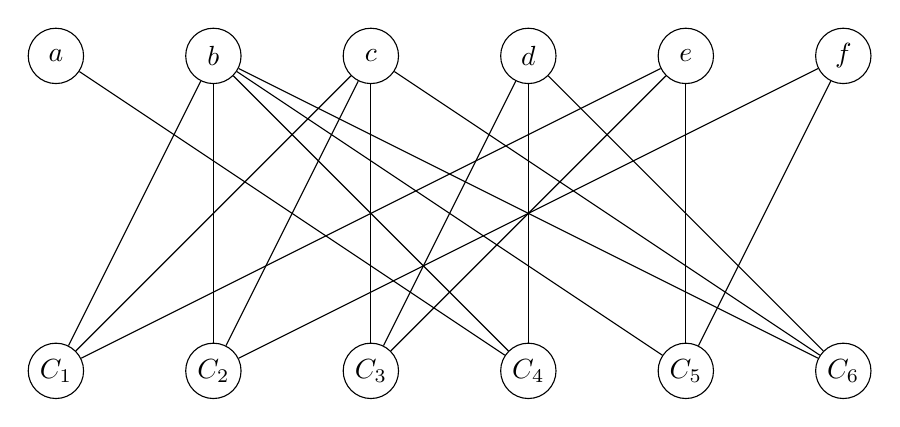
\begin{tikzpicture}
	\begin{scope}[auto, every node/.style={draw,circle,minimum size=2em,inner sep=1},node distance=2cm]
		\node[shape=circle,draw=black] (a) at (0,4) {$a$};
		\node[shape=circle,draw=black] (b) at (2,4) {$b$};
		\node[shape=circle,draw=black] (c) at (4,4) {$c$};
		\node[shape=circle,draw=black] (d) at (6,4) {$d$};
		\node[shape=circle,draw=black] (e) at (8,4) {$e$};
		\node[shape=circle,draw=black] (f) at (10,4) {$f$};
		\node[shape=circle,draw=black] (1) at (0,0) {$C_1$};
		\node[shape=circle,draw=black] (2) at (2,0) {$C_2$};
		\node[shape=circle,draw=black] (3) at (4,0) {$C_3$};
		\node[shape=circle,draw=black] (4) at (6,0) {$C_4$};
		\node[shape=circle,draw=black] (5) at (8,0) {$C_5$};
		\node[shape=circle,draw=black] (6) at (10,0) {$C_6$};
	\end{scope}
	\path [-](1) edge node {} (b);
	\path [-](1) edge node {} (c);
	\path [-](1) edge node {} (e);
	\path [-](2) edge node {} (b);
	\path [-](2) edge node {} (c);
	\path [-](2) edge node {} (f);
	\path [-](3) edge node {} (c);
	\path [-](3) edge node {} (d);
	\path [-](3) edge node {} (e);
	\path [-](4) edge node {} (a);
	\path [-](4) edge node {} (b);
	\path [-](4) edge node {} (d);
	\path [-](5) edge node {} (b);
	\path [-](5) edge node {} (e);
	\path [-](5) edge node {} (f);
	\path [-](6) edge node {} (b);
	\path [-](6) edge node {} (c);
	\path [-](6) edge node {} (d);
	
	\end{tikzpicture}
	\caption{Example preliminary graph $G_A$ on $\phi$}
	\label{fig:ga}
\end{figure}

\begin{figure}[h] 
		\captionsetup{justification=centering}
		
		\centering 
		\begin{tikzpicture}
		\begin{scope}[auto, every node/.style={draw,circle,minimum size=2em,inner sep=1},node distance=2cm]
			\node[shape=circle,draw=black] (b) at (0,4) {$b_T$};
			\node[shape=circle,draw=black] (bb) at (2,4) {$b_F$};
			\node[shape=circle,draw=black] (c) at (4,4) {$c_T$};
			\node[shape=circle,draw=black] (cc) at (6,4) {$c_F$};
			\node[shape=circle,draw=black] (e) at (8,4) {$e_T$};
			\node[shape=circle,draw=black] (ee) at (10,4) {$e_F$};
			\node[shape=circle,draw=black] (f) at (12,4) {$f_T$};
			\node[shape=circle,draw=black] (ff) at (14,4) {$f_F$};
			
			\node[shape=circle,draw=black] (1) at (0,0) {$C_1^1$};
			\node[shape=circle,draw=black] (2) at (2,0) {$C_1^2$};
			\node[shape=circle,draw=black] (3) at (4,0) {$C_1^3$};
			\node[shape=circle,draw=black] (4) at (6,0) {$C_1^4$};
			\node[shape=circle,draw=black] (5) at (8,0) {$C_2^1$};
			\node[shape=circle,draw=black] (6) at (10,0) {$C_2^2$};
			\node[shape=circle,draw=black] (7) at (12,0) {$C_2^3$};
			\node[shape=circle,draw=black] (8) at (14,0) {$C_2^4$};
		\end{scope}
		\path [-](1) edge node {} (bb);
		\path [-](1) edge node {} (cc);
		\path [-](1) edge node {} (ee);
		\path [-](2) edge node {} (b);
		\path [-](2) edge node {} (c);
		\path [-](2) edge node {} (ee);
		\path [-](3) edge node {} (b);
		\path [-](3) edge node {} (cc);
		\path [-](3) edge node {} (e);
		\path [-](4) edge node {} (bb);
		\path [-](4) edge node {} (c);
		\path [-](4) edge node {} (ee);
		\begin{scope}[>={Stealth[black]},
		every edge/.style={draw=red}]
		\path [-](5) edge node {} (bb);
		\path [-](5) edge node {} (cc);
		\path [-](5) edge node {} (ff);
		\path [-](6) edge node {} (b);
		\path [-](6) edge node {} (c);
		\path [-](6) edge node {} (ff);
		\path [-](7) edge node {} (b);
		\path [-](7) edge node {} (cc);
		\path [-](7) edge node {} (f);
		\path [-](8) edge node {} (bb);
		\path [-](8) edge node {} (c);
		\path [-](8) edge node {} (ff);
		\end{scope}   
		\end{tikzpicture}
	\caption{Snippet of example final graph $G_B$ on $\phi$.}{Only $C_1$ and $C_2$ is shown}
	\label{fig:gb}
\end{figure}

Professor Dawar's construction creates rigid graphs based off the $odd$ property of multipedes. The oddness property is replaced with check for unique satisfiability of an 3-XOR-Formula. Similarly the check for $k$-local consistency is replaced by identifying whether 3-XOR-Forumlas are solved quicker using Gaussian elimination operating within the algorithm, in comparison to the same formula without Gaussian elimination. In short, the check for oddness is replaced by unique satisfiability, thereby rendering them rigid, and the check for $k$-local consistency is estimated by comparing Gaussian elimination on and off times.

\newpage
\section[Solvers]{Solvers}
In order to construct our graphs, we will require multiple checks at different stages of construction. When we generate a random 3-XOR-Formula $\phi$, we need to ensure that it is $k$-locally consistent, uniquely satisfiable and gives rise to a preliminary graph with no automorphisms.  Checking for $k$-local consistency and unique satisfiability requires a SAT solving program to determine these attributes. Whereas a GI solver, namely Traces, is utilised to check for automorphisms.

\subsection[GI Solvers]{GI Solvers}
The programs Nauty and Traces are two of the fastest GI solvers for most cases of small and large graphs respectively. Nauty  was developed in the 1980s by B. Mckay \cite{mckay1981practical}, which was subsequently revised and incorporated into Traces \cite{mckay2014practical} in 2013. These programs utilise two key components in their algorithms: vertex colour refinement and factoring of graphs through found automorphisms.

Two main procedures provided by the Nauty and Traces are Automorphism Group ($Aut(G)$) and Canonical Labelling ($Canon(G)$) of graphs. Our work is concerned only with the $Aut(G)$ function, as graphs which execute slowly on $Aut(G)$ tend execute slowly on Canon(G) \cite{mckay2014practical}. These procedures are used to benchmark the performance of their algorithm, since the exact complexity of these programs is unknown. Additionally, since $Aut(G)$ shows us whether there are any automorphisms of a graph G, we use this feature in validating our preliminary graph $G_A$, as well as determining the performance of our final graph $G_B$.

The heuristic algorithm behind Nauty and Traces to determine graph isomorphism is a backtracking search which is based off two key elements: vertex colour refinement (also known as a 1-dimensional Weisfeiler-Leman test) and factoring graphs through found automorphisms \cite{mckay2014practical}. Our construction, being both rigid and resistant to Weisfeiler-Leman tests and its high dimensional variants, should be difficult for this algorithm.

\newpage
\subsection{SAT Solvers}
The algorithms behind SAT solvers typically use Gaussian Elimination in solving a system of linear equations. In some cases, this feature can be disabled, and some implementations do not use it all. By toggling Gaussian Elimination on and off, and recording the times, one can make a good guess at whether $\phi$ is $k$-locally consistent. Randomly generated systems which are solved significantly faster with Gaussian Elimination on versus off are ones of interest. The prediction is that systems with greater differences in execution speeds hints at $k$-local consistency of a system.

\section{Previous Attempt}
Recently, a study searched for the family of graphs Babai describes. E. Arrighi, a Cambridge intern guided by Prof. A. Dawar, the project supervisor, found that multipedes are theoretically complex for Traces. Arrighi concluded that the smallest examples of suitable probabilistically generated multipedes, containing significantly high probability of non-trivial automorphisms, would be too large to generate, so rendering them too large for experimentation on Traces. Instead, our approach utilised the same concepts from such hypergraphs, but constructs them in a smaller fashion.









%!TEX root = ../thesis.tex
%*******************************************************************************
%****************************** Third Chapter **********************************
%*****************************************\**************************************
\chapter{Requirements}
% **************************** Define Graphics Path **************************
% What would Anuj write?

\ifpdf
    \graphicspath{{Chapter3/Figs/Raster/}{Chapter3/Figs/PDF/}{Chapter3/Figs/}}
\else
    \graphicspath{{Chapter3/Figs/Vector/}{Chapter3/Figs/}}
\fi
The design of our program hinges on finding suitable constructions that match our criteria. Theoretically, two primary requirements must be met. Firstly, to find a set of equations (clauses), each of which contains three literals (variables), from a pool containing n elements. m is the number of equations within the formula. Hence, we must randomly generate a formula $\phi$, which has n literals and m equations, for specified values. $\phi$ must be both $k$-locally consistent and homogeneous. Secondly, to ensure that the set of equations $\phi$ must give rise to a construction, as defined in the Background segment, which has no non-trivial automorphisms. Thus, we will have constructed a graph that encapsulated CFI graphs and multipedes, proving resistant to the backtracking search of Traces.
\par
In this portion, we will consider what further requirements must be met, including defining our system conceptually, permitting us to take a reasoned step toward implementation. Furthermore, this allows the reader to reproduce our system without requiring much technical detail, permitting similar systems of different programming languages and so on. 

\section{Solvers}
Prior to defining system requirements, we must first consider the specification of tools we intend to invoke. Two programs are of importance. One is the GI solver, which we have already identified as Traces, and the other is a SAT solver, of which there are many implementations. To this end, we are able to use SAT solving competitions as a starting point. 

\subsection{Cryptominisat}
The international SAT solving competition is an annual meet where competitors pit their programs in a race to solve the SAT and UNSAT problem \cite{sat_competitions_2017}. Here lies a choice of open-source software to implement, all of which follow the same DIMACS specification of usage \cite{dimacs_2017}. Many are regularly maintained and well documented.
\par
Following the pre-implementation decision of using Python as a programming language of choice, we select Cryptominisat as our solver. Although this package is primarily written in C, it provides compact Python libraries to import and is well maintained on GitHub. Additionally, for reasons other than being awarded fastest solver in its track, we will describe how Cryptominisat can also be of great use in checking for $k$-local consistency and unique satisfiability.

\subsubsection{Input}
In order to comprehend how homogeneous systems are determined efficiently, we will first consider the DIMACS format previously mentioned. (For an elaborate explanation, see the DIMACS website. For our purposes, we will consider only special cases \cite{dimacs_2017}.)
\par
Input to the SAT solvers takes the form of text files. An example is shown below.
\begin{figure}[htbp!]
	\captionsetup{justification=justified, singlelinecheck=false}
	p cnf 4 5 \\
	1 3 4 0 \\
	2 -3 4 0 \\
	1 2 -4 0 \\
	1 -2 -3 0 \\
	-1 2 3 0 \\
	\caption{Example 3-XOR-Formula in DIMACS}
\end{figure}
\par
The first line defines the number of literals and the number of clauses in the cnf formula, 4 and 5 respectively. This is the equivalent of n and m as used in $\phi$. The following lines are cnf clauses. Each clause contains three literals, and is demarcated with the 0 value. Thus, line 2 denotes $(1 \lor 3 \lor 4)$, followed by line 3 stating $\land (2 \lor \lnot3 \lor 4)$ and so on. (Equivalently, $(a \lor c \lor d) \land (b \lor \lnot c \lor d)$). We can translate this syntax into more common mathematical system of equations and CNF formula:

\begin{figure}[htbp!]
	\centering
	\begin{minipage}{.4\textwidth}
		\begin{align*}
			a + c + d &= 1 \\
			b - c + d &= 1 \\
			a + b - d &= 1 \\
			a - b - c &= 1 \\
			-a + b + c &= 1 \\
		\end{align*}
	\end{minipage}
	$\iff$
	\begin{minipage}{.4\textwidth}
		\begin{align*}
			(a \lor c \lor d) \land \\
			(b \lor \lnot c \lor d) \land \\
			(a \lor b \lor \lnot d) \land \\
			(a \lor \lnot b \lor \lnot c) \land \\
			(\lnot a \lor b \lor c) \\
		\end{align*}    
	\end{minipage}
\end{figure}

Evidently, there is a satisfying value for these example: $a=0, b=1, c=0, d=1$ or $a=False, b=True, c=False, d=True$.
\par
Similarly, we have the following example input for an XOR-Formula, although CNF and XOR can be readily inferred from one another without the need to change syntax:
\begin{figure}[htbp!]
	\centering
	\begin{minipage}{.2\textwidth}
		p cnf 6 6 \\
		x2 3 5 0 \\
		x2 3 6 0 \\
		x3 4 5 0 \\
		x1 2 4 0 \\
		x2 5 6 0 \\
		x2 3 4 0 \\
	\end{minipage}
	$\iff$
	\begin{minipage}{.2\textwidth}
		\begin{align*}
			b + c + e &= 0 \\
			b + c + f &= 0 \\
			c + d + e &= 0 \\
			a + b + d &= 0 \\
			b + e + f &= 0 \\
			b + c + d &= 0 \\
		\end{align*}
	\end{minipage}
	$\iff$
	\begin{minipage}{.2\textwidth}
		\begin{align*}
			False(b \oplus c \oplus e) \land \\
			False(b \oplus c \oplus f) \land \\
			False(c \oplus d \oplus e) \land \\
			False(a \oplus b \oplus d) \land \\
			False(b \oplus e \oplus f) \land \\
			False(b \oplus c \oplus d) \land \\
		\end{align*}    
	\end{minipage}
\end{figure}

The notable difference in the syntax of the input is that we now prepend $x$ at the beginning of each line to demarcate an XOR clause. Note that this is also a homogeneous system that is uniquely satisfiable and gives rise to our desired construction $G_B$.
\par
This distinction is important as we have more than one method of validating unique satisfiability, which will ultimately effect the running time and space complexity of our algorithm. Specifically in searching for uniquely satisfiable set of clauses, that are on the threshold of satisfiability. As systems become larger, or closer to the threshold, the running time is expected to increase exponentially.

\subsubsection{Unique satisfiability}
Given Cryptominisat allows input in the form of mixed CNF and XOR clauses, we have to solutions to check for uniquely satisfiable and homogeneous solutions. We use uniquely satisfiable systems of equations as a replacement for the $odd$ property of multipedes, rendering them rigid. 
\par
Method A: Insert an additional XOR clause which contains a single literal. Then check for satisfiability. If for any of these literals there is a satisfying argument, then there is another solution to the system of equations which is not the all-zero solution. This is the only option if we are enforced to use strictly XOR clauses. However, Cryptominisat provides us the functionality of mixing XOR and CNF clauses.
\par
Method B: Insert an additional OR clause which contains all literals. Then check for satisfiability. If this statement is TRUE, then at least one literal must be TRUE for the statement to hold. Thus, there is another solution other than the all-zero solution.
\par
Both solutions have their caveats. The first solution would require $n$ repetitions to check for satisfiability. As these systems become large, validating a single system of equations may take a long period of time, but adds only small amount of complexity to the problem. Whereas the second solution would require that the XOR solver permit a combination of XOR systems and OR systems of different sizes, with one clause containing $n$ variables. This can be problematic as n becomes large complexity wise, but requires only one check. Depending on how the SAT solver manages, both options are available to test.

\subsubsection{$k$-local consistency}
The validation of $k$-local consistency of a system of equations is much more difficult than a simple check of a logical statement. 
\par
One way would be to locate uniquely satisfiable homogeneous systems which execute faster with Gaussian elimination working in the SAT solving algorithm, in contrast to the same system executing on a solver without this feature. Thus, we could compare a systems execution time on a SAT solver with Gaussian elimination to one without. Two separate algorithms would be required to make this comparison. Furthermore, Gaussian elimination is not central to these efficient algorithms, as we will see later. However, Cryptominisat does provide an option to build without this feature. Hence, rather than utilise two separate programs, we are able to build the same program twice with different algorithms. Thus eliminating the need to facilitate two separate packages, which will save implementation time.
\par
In checking $k$-local consistency using this feature, we would invoke Cryptominisat twice, once with "Gauss-On" and then with "Gauss-Off", on a uniquely satisfiable 3-XOR-Formula. We would take systems which execute faster with Gauss-On versus Gauss-Off. Those systems which have a larger discrepancy in times are deemed as more likely to be $k$-locally consistent, and would result in slower execution times as a construction. These are the systems which we are looking for.  

\newpage
\subsection{Traces}
Traces is our GI solver of choice. It has its own specifications of input, namely the DIMACS and \emph{Dreadnaut} standards. The graph constructions available on the Traces website are of these varieties, which are provided to reproduce benchmark tests and experiment with the suite \cite{piperno_2017}. We will use a number of these packages available to compare the performance of our construction. We intend to reproduce the benchmarks, and go further by involving more packages and extending the ones available, that is, creating larger instances of random graphs. Since we intend to execute numerous packages, we must implement an efficient way of executing them. Our goal is to run a family of graphs sequentially, and record execution times. Our construction will be packaged similarly to these graphs.

\subsubsection{Dreadnaut}
Executing graphs on Traces comes in a variety of implementations, however, we will be concerned with the well-documented and simple interface that is Dreadnaut. Dreadnaut is a tool that permits us to invoke both Nauty and Traces, with a variety of parameters. It is a command line tool provided in the Nauty/Traces suite which opens a shell for subroutines. Thus, we are able to invoke this tool by means of system class from our Python implementation. The major design issue is that we must use the \emph{.dre} (Dreadnaut) filetype in passing stored graphs as input, and not the generic DIMACS format. Therefore, in outputting our construction, we must adhere to this syntax.

\subsubsection{Benchmarks}
In reproducing benchmark tests, there is the issue of fairly testing graphs against one another. Hence, a suitable environment for executing constructions is required. For this issue, we consider using a machine that is uninterrupted by system processes. Traces does provide a means of accurately measuring execution times, however, this requires multiple executions of the same graph instance, which becomes costly as we increase the size of graphs. In addition, to attain sub-second timings, many repetitions must be executed to attain these values. This is problematic even for small graphs, where sub-second differences matter. Therefore, a makeshift method of recording times is presented, using the times of system calls. (Both Traces and system call times are captured in testing, which showed minor differences in times.) All packages are therefore timed in this manner on an external machine whose sole purpose is to conduct experiments. Moreover, many requirements produced in the benchmarks tended to run for very long periods of time, and had to be bounded by some timeout value. An appropriate value is chosen at the time of implementation. 

\section{Software Requirements}
Now that we have defined the requirements of the major tools utilized, we will describe the requirements of our implementation. These are more general issues, rather than design choices enforced by external software. Our product must meet these specified areas, in addition to the issues raised by tools. 

\subsection{Data Management}
We will be handling files in storing and executing our data, as well as the graphs provided by Traces. Hence, we will need to program our system to manipulate files, such as stored XOR-Formulas and constructions., which will be used as input to implemented tools. A database could be utilised, although, in our case, we will use the (Linux) filesystem as storage. This will allow us to transfer files as required, rather than having to persist in some datastore. It is important to ensure these files are stored, since locating difficult constructions will take time. The stored files will be provided along with our own package, which will be available as an open-source repository which also houses installation information \cite{quasipolynomial}.

\subsection{Reproducibility}
Ensuring that our results and findings are easily verifiable and reproducible, we provide a GitHub repository where all our work is publicly available. We intend to properly document our codebase, including instructions on how to install our package.
\par
As a requirement, we should be able to reproduce finding and constructing systems, execute graphs and benchmarks using Traces, and any other important discoveries we make. The constructions we find will be tend to the .dre specification, and will appear similar to one of the benchmark graph packages provided by Traces.

\subsection{Resources}
Our construction must be small enough to execute on Traces, yet be easy to find given the right parameters. Ideally, we would like our system to be located much faster than the execution time on Traces, so that we can build a database of constructions quickly. We therefore have two resource requirements: space and time, on our tools and system hardware.
\par
Traces is prone to exceed its allocated memory and crash or invoke thrashing of loading from secondary memory. Hence, we must keep this in mind when setting up our test server. Instances at given size will inevitably be too large for a system to handle in memory. 
\par
The outcome of executing systems on our SAT solver was unknown, however, we intended to implement a timeout similar to the one utilised in Traces benchmarks. This can be problematic as we will require multiple runs to locate $k$-locally consistent systems, so some upper bound must be put in place for an efficient search. Enough memory and a time bound must be provided for both of our tools, which will be manipulating our constructions. Both in searching for constructions and executing constructions, we expect to reach execution times within the scale of hours. Hence, one can expect some very difficult instances or a group of instances to take many days to execute. Moreover, it is unknown how it will take to find suitable systems at large values of $m$ and $n$. We expect a sparse amount along the threshold of satisfiability. Hence, searching, validating and executing graphs and systems will take a long period of time. This is why a process must remain uninterrupted for many days on our test server. 






%%!TEX root = ../thesis.tex
%*******************************************************************************
%****************************** Third Chapter **********************************
%*******************************************************************************
\chapter{Design and Implementation}

% **************************** Define Graphics Path **************************
\ifpdf
    \graphicspath{{Chapter3/Figs/Raster/}{Chapter3/Figs/PDF/}{Chapter3/Figs/}}
\else
    \graphicspath{{Chapter3/Figs/Vector/}{Chapter3/Figs/}}
\fi

Moving onward from our requirements, we take the first step in producing our final product. Prior to development however is the setup of our working environment, which is of importance if we are to describe the issues and choices in development, preventing or influencing capabilities. We leave much of the directory structure and information on where results are stored and how they can be reproduced in our GitHub repository \cite{quasipolynomial}.

\section[Development Environment]{Development Environment}
Our development setup is shown in Table \ref{tab:t1}. Evidently, we have enough hardware capabilities to meet the baseline requirements of our tools. However, this still led to issues described in later segments, including out of memory errors and erroneous execution times. Although, we did not experience all errors on our test server. 

\begin{table}
	\caption{Development Setup}
	\centering
	\label{table:good_table}
	\begin{tabular}{l l}
		\toprule
		Feature & Description  \\ 
		\midrule
		Operating System & Ubuntu 16.10 64-bit \\
		Programming Language &  Python 2.7\\
		Programming Language Tools & numpy, timeit, matplotlib\\
		Command Line Tools & dreadnaut, nauty/Traces \\
		Versioning & Github (Public Repo) \\
		RAM & 8GB DDR3 \\
		Disk & 500GB ATA SanDisk Ultra II SSD \\
		CPU & 8 x Intel Core i7-3612QM CPU @ 2.10GHz \\
		\bottomrule
	\end{tabular}
	\label{tab:t1}
\end{table}



\section[Architecture]{Architecture}
Our system setup separates development and experiment stages of our program. We first created our package on a laptop computer, which would regularly update experiments, data and code through SSH, FTP and GitHub respectively. Once experiments were completed, we would save these results to our repository and then generate plots. This was to esnure that the python process in action would remain undisturbed by any other system process. Both systems used a form of Linux, and the experiment server was hoster on Digital Ocean, which allowed us to change system resources as required. This is important to note as we frequently had to do this.
\par
\begin{figure}[htbp!]
	\begin{center}
		\leavevmode
		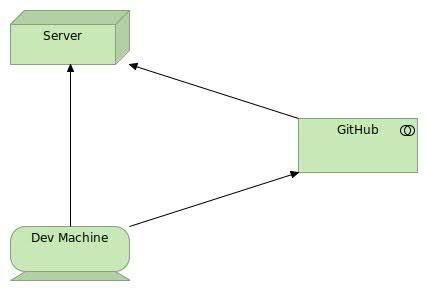
\includegraphics[height=50mm]{Figs/architecture.jpg}
	\end{center}
	\caption{System Architecture}
	\label{fig:one}
\end{figure}
\begin{figure}[htbp!]
	\begin{center}
		\leavevmode
		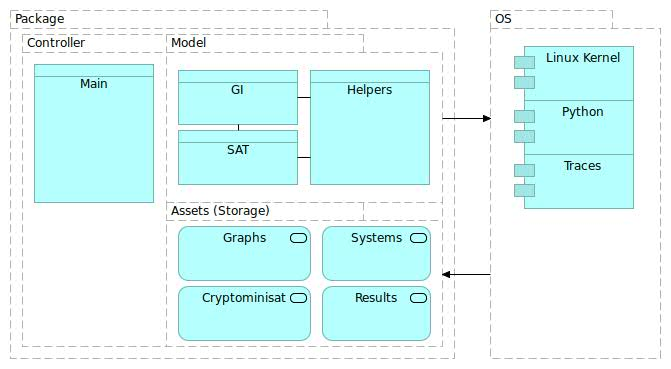
\includegraphics[height=50mm]{Figs/implementation-architecture.jpg}
	\end{center}
	\caption{Software Architecture}
	\label{fig:one}
\end{figure}

\section{Algorithms}
We two major steps in our program: locating our desired systems, and then converting them to our construction. With the added stages of separating graphs into packages which varied in complexity, and then executing these graphs to find execution times, we have a total of four key steps. The following diagram depicts our workflow:

\begin{figure}[h]
	\centering
	\begin{tikzpicture}[
	node distance = 5mm and 7mm,
	start chain = going right,
	alg/.style = {draw, align=center, font=\linespread{0.8}\selectfont}
	]
	\begin{scope}[every node/.append style={on chain, join=by -Stealth}]
	\node (n1) [alg] {Find \\ systems};
	\node (n2) [alg]  {Convert \\ to graphs};
	\node (n3) [alg]  {Seperate \\ into packages};
	\node (n4) [alg] {Benchmark \\ tests};
	\end{scope}
	\end{tikzpicture}
	\caption{Typical workflow}
	
	
\end{figure}
Each stage has its own form of elaborate checks and logic. Here we will describe each part does, how it is integrated into our architecture and notable pieces of logic. Note that this is the most basic usage of our software, and additional features and options are mentioned later. We will only describe the first two parts here, and the second parts in the Evaluation, as the following steps were a result of findings. 

\subsection{Timing}
Times were monitored using pythons Timeit library. If a timeout was specified, and exception would be thrown and handled appropriately. Runs which required the uses of system calls, such as dreadnaut and Traces, would be called using the Process Handler. One would record the time before and after the call was made. Granted this does not give the very accurate times, but was satisfactory enough to gauge the general idea. We assumed that making the system call would only add sub second times to overall execution, which results in no large changes in the execution of large graphs, which executed for multiple minutes. 
\newpage
\subsection[Systems Search]{Systems Search}
Given values max\_n	and max\_m, the maximum number of clauses and literals respectively, we search for systems in the following manner (see algorithm for details): let $n=m=4$; iterate over the set $N=\{n, n+step,..,max\_n\}$; for each $n \in N$, iterate over the set $M=\{m, m+step,..,max\_m\}$; for these values of $n$ and $m$, generate a random system of equations from a pool of $n$ literals, that is $\{1,2,..,n\}$ with $m$ clauses; validate this system for unique satisfiability and k-local consistency; if it is valid, then store this system. See Algorithm \ref{alg:a1}.
\par
There are, of course, many checks not mentioned, however, we take this as the simplest form of generating a range of systems, over the Cartesian product of $N$ and $M$, where $n \leq m$. Thereby ranging from the line of satisfiability, $n=m$, to some $n=max_n$ and $m=max_m$

\begin{algorithm}[htbp!]
\SetAlgoNoLine
\KwIn{Integers $min\_n$, $min\_m$, $max\_n$, $max\_m$, $step$, $max\_tries$.}
\KwOut{A set of uniquely satisfiable and k-locally consistent XOR-Formulas.}
$systems = \{\}$\;

\Repeat{$min\_n$ == $max\_n$}{
	$tries = 0$\;
	
	\Repeat{$min\_m$ == $max\_m$}{
		\If{$tries == max\_tries$}{
			$tries = 0$\;
			$min\_m += step$\;
			skip this iteration\;
		}
		
		$system$ = Generate random system($min\_n, min\_m$)\; 
		\eIf{system is uniquely satisfiable and k-locally consistent($system$)}{
			$systems$ add $system$\;
			$tries = 0$ \;
			$min\_m +=step$\;
		}{
		$tries += 1$\;
	}	
}
$min\_n += step$\;
}

return $systems$
\caption{Fundamental Search: Finding uniquely satisfiable and k-locally consistent systems}
\label{alg:a1}
\end{algorithm}

\newpage
\subsection{Constructing Graphs}
In transforming eligible systems into our final construction, we must first ensure that the graphical representation of our XOR-Formula contains no automorphisms. This is determined by Traces, and is fairly easy to compute. Recall in the background segment we label the preliminary and final graphs $G_A$ and $G_B$ respectively. See Algorithm \ref{alg:a2}.
\par
$G_A$ is trivial to construct into its graphical representation, whereas $G_B$ requires only slightly more logic. We used numpy matrices to construct adjacency matrices from a system, which worked sufficiently well for large systems. 
\begin{algorithm}[htbp!]
		\SetAlgoNoLine
		\KwIn{Integers $n$, $m$.}
		\KwOut{A set of random 3 literal clauses}
		$pool = \{1,2,..,n\}$\;
		$system=\{\}$\;
		$tries=3$\;
		$index=0$\;
		
		\Repeat{$index$ == $m$}{
			\If{$tries==0$}{
				return $False$\;
			}
			$clause$ = random 3 literals from $pool$\;
			\eIf{$clause \in system$}{
				$tries-=1$\;
			}{
			$system$ add $clause$\;
			$index+=1$\;
		}
	}
	
	return $systems$
	\caption{Generate random system}
	\label{alg:a2}
\end{algorithm}



\newpage
\section{Parameter Settings}
During implementation, many constants and variables were assigned values in response to issues. These hard coded values are of importance when we discuss results. For the meantime, we will define them here so that they can easily be identified. See the following table for descriptions.

\begin{table}[h]
	\centering
	\label{tab:parm}
	\begin{tabular}{p{2cm}| p{11cm}}
		\toprule
		Parameter & Description \\
		\midrule
		Step & Searching for systems requires some iterator over n and m. This increments m by some value. \\ \hline
		Limit &  We may want to find this number of systems from a given m. Useful if we want to find the smallest ratios. \\ \hline
		Tries & Generating random systems has two problems: 1, we include the same clause twice from a pool of literals. 2, The system may not match our criteria Therefore, we try this many times before moving on.\\ \hline
		Timeout & dreadnaut, nauty/Traces \\ \hline
		Upper bound and lower bound & Suppose we wanted to search along the threshold of satisfiability. we would set this value to 1. This describe the upper and lower bound of n = u * m, for some u.\\ \hline
		Strongly $k$ & A system is strongly $k$ if there is a large difference in Gauss-On versus Gauss-Off. Some systems have a larger discrepancy than others of the same size. We put aside systems with the largest discrepancy during our Advanced Search. \\ \hline
		\bottomrule
	\end{tabular}
	\caption{Search parameters}
\end{table}
\newpage
\section{Development Issues}
Faults are inevitable in ever undertaking, and ours are reported in this segment.
\par
We noticed during execution strange behaviour from Traces and the operating system. This is notable  since these issues may effect our report of results, although, these issues may be uncommon and spurious. 

\subsection{Python OOM}
Python processed tended to crash after short periods of time on the experiment server. This required swap space to be allocated as RAM was not satisfactory. Attempts were made without having to include swap space, the caveats being access to secondary memory should be averted. However, larger implementations which included a 2 CPU machines with 2gb RAM still was not satisfactory. Therefore, swap space must be included on small installations. 

\subsection{Traces OOM and Indefinite Execution}
Traces was expected to halt when instances became too large to process. Luckily, our construction was below this threshold for small instances that mattered. However, at node sizes roughly at 6000, Traces began to fall short at seemingly random times. Occasionally, Traces would run one graph for an indefinite period of time (which had to be manually cancelled), and for another run, ran for a few hours. Given that we had the instances we needed, this issue was not explored, and may have only been an operating system issue, since 20gb swap space had to be allocated to permit for larger instances.
\par
For some instances, even at the relatively small end of our graphs, which consisted of a manageable number of nodes, say 4000, Traces would crash unexpectedly after multiple hours. The details of these instances were not recorded, however for relatively small values of our graphs, graphs which executed for numerous hours, say n=500, Traces would fail. It is unknown whether this due to hardware insufficiencies. Therefore, for instances which timeout, where no timeout is defined - this describes a system error of some sort. One such example is the tnn(2) graph, whose similar graph tnn(1), would run for multiple days, causing strange CPU behaviour. There is a picture of this issue displayed in appendix. The cause is unknown, a snapshot of the development server is also placed in the appendix to reproduce problems. Hence, some instances which timed out, may have in fact fell under this bug. It is quite possible that instances became too complex at a point, which required more swap space than allocated. However, this is only a speculation.

\section{Additional Features}
Given that there is more than one way to program our logic, multiple strategies were used to generate our desired construction. Here we define additional methods utilised and features that extended beyond our requirements and design. They may be of importance in future applications.

\subsection{Alternative XOR-Formula Generation}
Our algorithm to generate desired systems picks three random literals and adds these to a set of clauses. However, for some values of $n$ and $m$, a system cannot be located. We know that there exists a suitable system for these values, but cant be selected at random due to the large permutation of $n$. For small values of $n$ and $m$, we believed that all combinations could be held in memory and systematically tested, rather than being generated at random. Hence, a recursive search is provided to find all combinations to be tested. However, in implementation, this could not be used even for small values of n and m due to running times. Nonetheless, this feature may be of importance when time is not an issue, and a set of desired systems are required for given values.

\subsection{Updating Slow Systems}
Since we determine $k$-local consistency by checking if one system executes faster with Gauss-On versus Gauss-Off, it can be problematic to determine if a system is suitably slow. Small systems execute very quickly, and differ into two runs by only sub second values. These sub second difference could be mistaken for fluctuations in system performance, rather actual operating time (since we are measuring time not by process execution time, but start and end times). Here we have two solutions to mitigate this error.
\par
The first solution is to use some parameter, say \emph{minimal\_difference}, to provide a lower bound on the value required for a $k$-locally consistent system. However, this may be too large for small systems to register or too small to attain difficult instances. The second option is to solve this problem by repeating runs. We save those systems which have the largest difference in a separate directory, and replace these systems when comparing differences. If a newly found system is slower, that is it has a larger positive difference than the stored one, then we replace the stored one. This way, by using many iterations, we can generate a set of systems which have the largest differences to date. We are able to filter out those instances with exceptionally slow times. These graphs will be the most difficult found, and thus, the ideal type to construct to use in benchmarking. We prove this experimentally.

\subsection{Advanced Search}
Considering that we must check if a suitable system gives rise to a graph with no non-trivial automorphism, we can combine this check when searching for systems. In addition to updating strongly k-systems, we have the tools to search for the ideal graph.
\par
If we convert the system to a graph and check for automorphisms on the fly, that is, whilst searching and validating systems, we eliminate the need to build up a database of suitable systems up to the point of automorphisms, at the cost of running time. There are parameters defined enabling us to use this extended validation check.

\subsection{Optimised Search}
Numerous parameters are available to speed up searching. Here we briefly describe how they can be used.
\par
The upper bound and lower bound variables search for a given region of $n and m$. For example, if we wanted to search for systems along the line of satisfiability, we would set both values to 1. This would ensure we get the most difficult instances possible, but results in longer execution time due to failed tries. Moreover, we can check along $2n=m$ or between $n=m$ and $2n=m$, and so forth. This becomes clear in the following Chapter.
\par
Similar to the upper bound and lower bound variables, the limit variable permits us to search for a given number of systems for a given n. That is, move up n by step if we have found $limit$ systems. This is important when we consider the next paragraph.
\par
Efficient search variable checks that we solve the following optimisation problem. If we begin by searching along the line n=m, for large n, and no such system was found up until n=2m, then it is unlikely that the following iteration $n=n+step$ will find a system between n=m and n=2m. Thus, efficient search remembers the last good m value. Thereby eliminating the need to make redundant checks. This is useful, for suppose we set limit=1, lower-bound = upper-bound = 1, tries = 1000, $update\_strongly\_k = true$, then we could efficiently find systems close the the threshold of satisfiability. A number of these example searches are provided in the appendix. 
 \newpage
\subsection{Extending Traces Benchmarks}
To permit us to see how large we could potentially make out construction, numerous random graphs provided by Traces were extended. Graphs with edge probability 1/2, 1/10 and sqrt(n) were constructed using programs provided by the nauty/Traces suite: genrang (to build) and showg (to convert .g6 to .dre). Instances ranged from 5 to 30,000 nodes, and were executed successfully.

%%!TEX root = ../thesis.tex
%*******************************************************************************
%****************************** Third Chapter **********************************
%*******************************************************************************
\chapter{Evaluation}

% **************************** Define Graphics Path **************************
\ifpdf
    \graphicspath{{Chapter3/Figs/Raster/}{Chapter3/Figs/PDF/}{Chapter3/Figs/}}
\else
    \graphicspath{{Chapter3/Figs/Vector/}{Chapter3/Figs/}}
\fi

We evaluate our system in two parts: evaluation of program performance, and then how our construction did. Once defined, we will elaborate on results on various findings. Firstly, we will define our tested and the performance of benchmark graphs provided by Traces. For results which were not crucial to this project, see our GitHub repository \cite{quasipolynomial}. 

\section{Testing Environment}
Our experiments were conducted on a cloud computer server to ensure long-running processes, such as searching and executing families of graphs, remained undisturbed. We often had to resize and make adjustments to system resources, as computing with our instances became difficult, as well as some benchmark graphs. We had the following setup.

\begin{table}[h]
	\caption{Test Environment}
	\centering
	\label{table:test_env}
	\begin{tabular}{l l}
		\toprule
		Feature & Description  \\ 
		\midrule
		Host & DigitalOcean \\
		Operating System & Ubuntu 16.10 64-bit \\
		Memory & 2GB \\
		Disk & 20GB SSD \\
		CPU & 2 CPUs \\
		Swap space & 4GB \\
		Programming Language &  Python 2.7\\
		Command Line Tools & dreadnaut, nauty/Traces \\
		\bottomrule
	\end{tabular}
\end{table}

Note that we had to allocate 4GB swap space to tackle large instances to accommodate both Python and Traces memory requirements. A good tutorial is here:\\ https://www.digitalocean.com/community/tutorials/how-to-add-swap-on-ubuntu-14-04

\section{Benchmark Tests}
In gaining insight of the performance of our graphs, we first describe what results were reproduced. In total, we tested a suite of 33 graphs for the Automorphism Group function of Traces, more than what was necessary to determine our performance. We will now describe a few interesting packages worth mentioning; graphs we extended, slow graphs and interesting graphs. The graphs here mentioned are of most importance, additional benchmarks are provided in the appendix. For additional information about these graphs, refer to the Traces website. All graphs had a timeout value of three hours.

\subsubsection{Random Graphs}
Knowing that Traces may run out of memory, and in part, the most intuitive graph we can compare to are random graphs with differing edge probabilities. Our construction is also generated at random, but with a much more sophisticated algorithm. So random graphs provided a starting point for comparison and testing the capabilities of Traces.

The random graphs provided by Traces differed in edge probabilities: 1/2, 1/10 and sqrt(n), where n is the number of vertices. that is to say, given a number of nodes n, add edges with the probabilities to each pair of nodes with edge probabilities above. The sizes of these graphs however, was somewhat small, ranging up to 5000 nodes. In practice, these executed the Automorphism Group test of Traces quickly. We then made it our business to extend up to 30,000 nodes to see what would happen.

\begin{figure}[htbp!] 
	\centering
	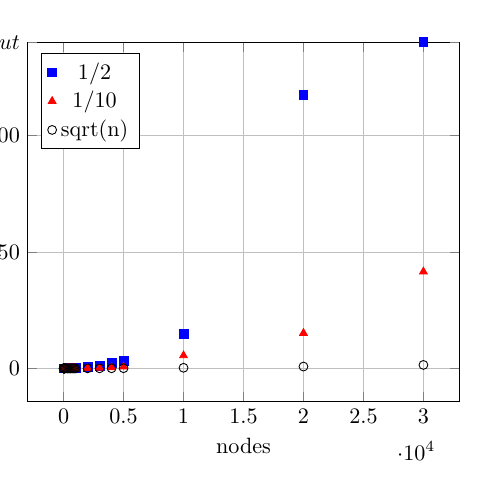
\begin{tikzpicture}[trim left=0cm, scale=0.8]
	\begin{axis}[
		xlabel=nodes,
		ylabel=t sec,
		legend pos=north west,
		grid=both,
		  extra y ticks={140},
		  extra tick style={grid=major, grid style={dotted, cyan}},
		  extra y tick labels={\hspace{5em}$timeout$},
		  extra x tick labels={},
		  extra y tick style={grid=none},
		  ymax=140
	]
	\addplot[
		scatter,only marks,scatter src=explicit symbolic,
		scatter/classes={
		  	a={mark=square*,blue},
		  	b={mark=triangle*,red},
		  	c={mark=o,draw=black,fill=black}
		}
	]
	table[x=x,y=y,meta=label]{
	  	x    y    label
	  	5	0.000801086425781	a
	  	10	0.000857830047607	a
	  	15	0.000815868377686	a
	  	20	0.00086498260498	a
	  	25	0.000833034515381	a
	  	30	0.000885009765625	a
	  	40	0.00108909606934	a
	  	50	0.000993013381958	a
	  	60	0.00110292434692	a
	  	70	0.00121307373047	a
	  	80	0.0013689994812	a
	  	100	0.00164794921875	a
	  	200	0.00490808486938	a
	  	300	0.0093150138855	a
	  	400	0.0167360305786	a
	  	500	0.0253059864044	a
	  	600	0.057608127594	a
	  	700	0.0520691871643	a
	  	800	0.0675909519196	a
	  	900	0.0881798267365	a
	  	1000	0.10640001297	a
	  	2000	0.486861944199	a
	  	3000	1.15394091606	a
	  	4000	2.44690203667	a
	  	5000	3.31565213203	a
	  	10000	14.8829817772	a
	  	20000	117.417869091	a
	  	30000	140 a
	  	5	0.000885009765625	b
	  	10	0.000794172286987	b
	  	15	0.000741004943848	b
	  	20	0.000755786895752	b
	  	25	0.000725984573364	b
	  	30	0.000759124755859	b
	  	40	0.000608921051025	b
	  	50	0.000768899917603	b
	  	60	0.000777959823608	b
	  	70	0.00056004524231	b
	  	80	0.000833034515381	b
	  	100	0.000924110412598	b
	  	200	0.00145792961121	b
	  	300	0.00253701210022	b
	  	400	0.00378179550171	b
	  	500	0.00561785697937	b
	  	600	0.00787591934204	b
	  	700	0.0102968215942	b
	  	800	0.0132210254669	b
	  	900	0.0209939479828	b
	  	1000	0.0328350067139	b
	  	2000	0.092490196228	b
	  	3000	0.217137813568	b
	  	4000	0.437031030655	b
	  	5000	0.702178001404	b
	  	10000	5.52752995491	b
	  	20000	15.1563310623	b
	  	30000	41.5227429867	b
	  	5	0.00109505653381	c
	  	10	0.000798940658569	c
	  	15	0.000815153121948	c
	  	20	0.000773906707764	c
	  	25	0.000853061676025	c
	  	30	0.000845909118652	c
	  	40	0.000874042510986	c
	  	50	0.000829935073853	c
	  	60	0.000848054885864	c
	  	70	0.000916004180908	c
	  	80	0.00099515914917	c
	  	100	0.00124502182007	c
	  	200	0.00164079666138	c
	  	300	0.00241208076477	c
	  	400	0.00246500968933	c
	  	500	0.00314116477966	c
	  	600	0.0039529800415	c
	  	700	0.00449395179749	c
	  	800	0.00527095794678	c
	  	900	0.00981688499451	c
	  	1000	0.00788497924805	c
	  	2000	0.0212609767914	c
	  	3000	0.0376129150391	c
	  	4000	0.0647239685059	c
	  	5000	0.0853998661041	c
	  	10000	0.264319896698	c
	  	20000	0.797810077667	c
	  	30000	1.4938249588	c
	};
	\legend{1/2, 1/10,sqrt(n)}
	\end{axis}
	\end{tikzpicture}
	
	\caption{Extended random graphs up to 30,000 nodes}
\end{figure}

\newpage
\subsubsection{Cai-Furer-Immerman Graphs}
Another notable graph family are the Cai-Furer-Immerman graphs, also known as CFI. These constructions are resistant to the 1-dimensional Weisfeller-Lehman tests and variants, but are prone to being factored by automorphisms in Traces. See Figure \ref{fig:cfi}.

\subsubsection{Other Graphs}
Other notable graphs which we include here are graphs which were amongst the slowest executing. These include Hadamard (had), Disjoint union of triparite graphs (tnn) and projective planes of order 25 (pp). Note that on the $x$ axis of pp graphs we select only the graphs which have 1302 nodes. thus, the $x$ axis only represents the label of the graph.

\begin{figure}[htbp!]
	\centering
	\begin{minipage}{.4\textwidth}
		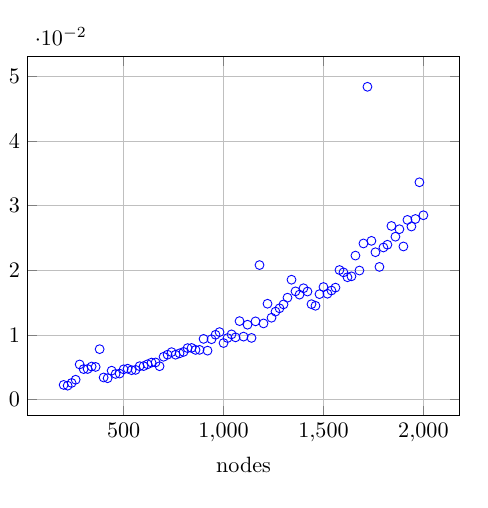
\begin{tikzpicture}[trim left=0cm, scale=0.8]
		\begin{axis}[
		xlabel=nodes,
		ylabel=t sec,
		grid=both
		]
		\addplot[
		scatter,only marks,scatter src=explicit symbolic,
		scatter/classes={
			a={mark=o,blue}
		}
		]
		table[x=x,y=y,meta=label]{
			x    y    label
			200	0.00228190422058	a
			220	0.00216603279114	a
			240	0.0025839805603	a
			260	0.00308394432068	a
			280	0.00544500350952	a
			300	0.00472712516785	a
			320	0.00474214553833	a
			340	0.00512409210205	a
			360	0.0050630569458	a
			380	0.00780987739563	a
			400	0.00343179702759	a
			420	0.00331783294678	a
			440	0.00448203086853	a
			460	0.00397682189941	a
			480	0.0040340423584	a
			500	0.0046911239624	a
			520	0.00479102134705	a
			540	0.0045599937439	a
			560	0.00460505485535	a
			580	0.00517892837524	a
			600	0.00519204139709	a
			620	0.00547194480896	a
			640	0.00573587417603	a
			660	0.0057520866394	a
			680	0.00517296791077	a
			700	0.0066339969635	a
			720	0.00695490837097	a
			740	0.00734996795654	a
			760	0.00695300102234	a
			780	0.00716400146484	a
			800	0.00738596916199	a
			820	0.00797080993652	a
			840	0.00799918174744	a
			860	0.00769591331482	a
			880	0.00770401954651	a
			900	0.00939702987671	a
			920	0.00758194923401	a
			940	0.00934600830078	a
			960	0.0100378990173	a
			980	0.0104479789734	a
			1000	0.00875687599182	a
			1020	0.00953316688538	a
			1040	0.010097026825	a
			1060	0.00963497161865	a
			1080	0.0121469497681	a
			1100	0.00975108146667	a
			1120	0.0115921497345	a
			1140	0.00955009460449	a
			1160	0.0121080875397	a
			1180	0.0208129882812	a
			1200	0.0117888450623	a
			1220	0.0148329734802	a
			1240	0.0126678943634	a
			1260	0.0136151313782	a
			1280	0.0141289234161	a
			1300	0.0147290229797	a
			1320	0.0157740116119	a
			1340	0.0185480117798	a
			1360	0.0167479515076	a
			1380	0.0162441730499	a
			1400	0.0172300338745	a
			1420	0.0167219638824	a
			1440	0.0147659778595	a
			1460	0.0145189762115	a
			1480	0.0163161754608	a
			1500	0.0174181461334	a
			1520	0.0163819789886	a
			1540	0.0168778896332	a
			1560	0.0173258781433	a
			1580	0.0200490951538	a
			1600	0.0196859836578	a
			1620	0.0189318656921	a
			1640	0.019070148468	a
			1660	0.0222799777985	a
			1680	0.0199689865112	a
			1700	0.0241541862488	a
			1720	0.0483820438385	a
			1740	0.0245571136475	a
			1760	0.0227990150452	a
			1780	0.0205280780792	a
			1800	0.0235340595245	a
			1820	0.0239598751068	a
			1840	0.0268609523773	a
			1860	0.0251989364624	a
			1880	0.0263600349426	a
			1900	0.0236899852753	a
			1920	0.0277979373932	a
			1940	0.0267760753632	a
			1960	0.027941942215	a
			1980	0.0336151123047	a
			2000	0.0285170078278	a
		};
		\end{axis}
		\end{tikzpicture}
		
	\end{minipage}
	\begin{minipage}{.4\textwidth}
		\centering
		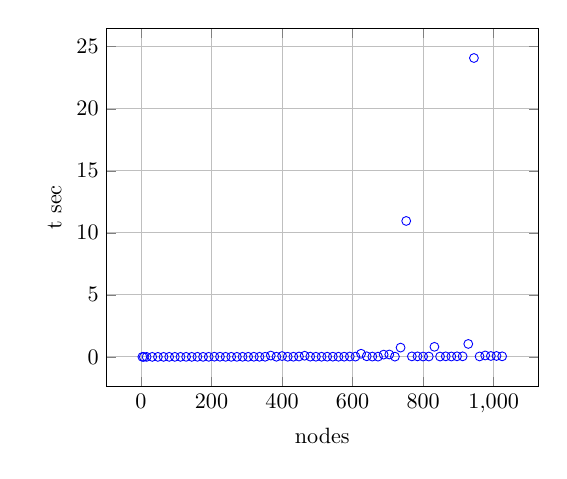
\begin{tikzpicture}[trim left=-1cm, scale=0.8]
		\begin{axis}[
		xlabel=nodes,
		ylabel=t sec,
		grid=both
		]
		\addplot[
		scatter,only marks,scatter src=explicit symbolic,
		scatter/classes={
			a={mark=o,blue}
		}
		]
		table[x=x,y=y,meta=label]{
			x    y    label
			4	0.000930070877075	a
			8	0.000865936279297	a
			16	0.000845193862915	a
			32	0.000930786132812	a
			48	0.00147294998169	a
			64	0.00136494636536	a
			80	0.00255489349365	a
			96	0.00285792350769	a
			112	0.00303387641907	a
			128	0.00530004501343	a
			144	0.00288701057434	a
			160	0.00666308403015	a
			176	0.00345611572266	a
			192	0.00493788719177	a
			208	0.0167338848114	a
			224	0.0145990848541	a
			240	0.00622987747192	a
			256	0.00490307807922	a
			272	0.00505113601685	a
			288	0.00681591033936	a
			304	0.00606393814087	a
			320	0.0118939876556	a
			336	0.0076220035553	a
			352	0.0107100009918	a
			368	0.1057908535	a
			384	0.0120139122009	a
			400	0.0673158168793	a
			416	0.0125169754028	a
			432	0.0138850212097	a
			448	0.0296130180359	a
			464	0.093101978302	a
			480	0.0204088687897	a
			496	0.0136818885803	a
			512	0.0128610134125	a
			528	0.017657995224	a
			544	0.0184848308563	a
			560	0.0129160881042	a
			576	0.0185670852661	a
			592	0.0293200016022	a
			608	0.0233659744263	a
			624	0.253060817719	a
			640	0.0492939949036	a
			656	0.0243890285492	a
			672	0.0193901062012	a
			688	0.183281898499	a
			704	0.194499969482	a
			720	0.0207889080048	a
			736	0.749053001404	a
			752	10.9565410614	a
			768	0.0408179759979	a
			784	0.0409290790558	a
			800	0.029314994812	a
			816	0.0302150249481	a
			832	0.811336994171	a
			848	0.0284330844879	a
			864	0.0446970462799	a
			880	0.0330929756165	a
			896	0.0468261241913	a
			912	0.0451979637146	a
			928	1.04390501976	a
			944	24.0905220509	a
			960	0.0360689163208	a
			976	0.116590023041	a
			992	0.0725729465485	a
			1008	0.0731618404388	a
			1024	0.0454850196838	a
		};
		\end{axis}
		\end{tikzpicture}
	\end{minipage}
	\captionsetup{justification=centering}
	\caption{Left: Cai-Furer-Immerman graphs (cfi).
		Right: Hadamard (had). }
	
	\label{fig:cfi}
\end{figure}
\begin{figure}[htbp!] 
	\centering
	\begin{minipage}{.4\textwidth}
		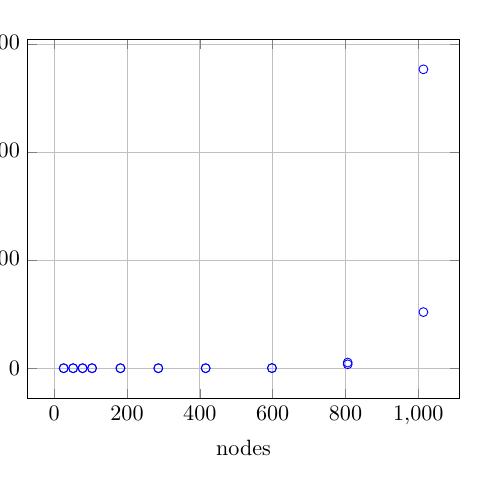
\begin{tikzpicture}[trim left=0cm, scale=0.8]
		\begin{axis}[
		xlabel=nodes,
		ylabel=t sec,
		grid=both
		]
		\addplot[
		scatter,only marks,scatter src=explicit symbolic,
		scatter/classes={
			a={mark=o,blue}
		}
		]
		table[x=x,y=y,meta=label]{
			x    y    label
			26	0.000897169113159	a
			26	0.000981092453003	a
			52	0.0010359287262	a
			52	0.00107097625732	a
			78	0.00181889533997	a
			78	0.00164103507996	a
			104	0.00313401222229	a
			104	0.00259685516357	a
			182	0.0143599510193	a
			182	0.0137579441071	a
			286	0.0655310153961	a
			286	0.0696680545807	a
			416	0.350058078766	a
			416	0.397336959839	a
			598	2.66647791862	a
			598	2.50128698349	a
			806	72.1839659214	a
			806	104.950797796	a
			1014	1039.76025891	a
			1014	5536.82137489	a
		};
		\end{axis}
		\end{tikzpicture}
		
	\end{minipage}
	\begin{minipage}{.4\textwidth}
		\centering
		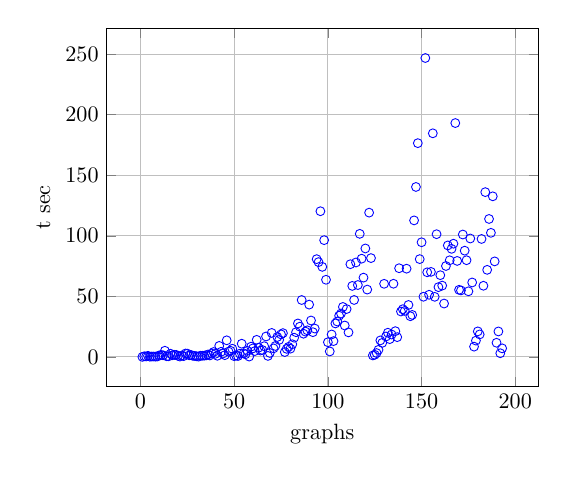
\begin{tikzpicture}[trim left=-1cm, scale=0.8]
		\begin{axis}[
		xlabel=graphs,
		ylabel=t sec,
		grid=both
		]
		\addplot[
		scatter,only marks,scatter src=explicit symbolic,
		scatter/classes={
			a={mark=o,blue}
		}
		]
		table[x=x,y=y,meta=label]{
			x    y    label
			1	0.0126891136169	a
			2	0.506518125534	a
			3	0.392946004868	a
			4	0.894825935364	a
			5	0.196982145309	a
			6	0.315265893936	a
			7	0.332309007645	a
			8	0.24335193634	a
			9	0.365062952042	a
			10	1.23158407211	a
			11	1.57859182358	a
			12	1.39838004112	a
			13	5.08932209015	a
			14	0.509947776794	a
			15	0.502409934998	a
			16	2.62835597992	a
			17	1.43174910545	a
			18	1.66480398178	a
			19	1.67586994171	a
			20	0.863186120987	a
			21	0.319430112839	a
			22	1.08262300491	a
			23	0.651422977448	a
			24	2.7789580822	a
			25	2.71859312057	a
			26	1.33379912376	a
			27	1.57668685913	a
			28	0.861810922623	a
			29	0.814624786377	a
			30	0.491320848465	a
			31	0.250020027161	a
			32	0.979526042938	a
			33	0.990874052048	a
			34	1.03750896454	a
			35	1.27122998238	a
			36	1.9730348587	a
			37	1.21517491341	a
			38	2.7824409008	a
			39	4.03445410728	a
			40	2.57081913948	a
			41	0.918713092804	a
			42	9.09311699867	a
			43	4.21852302551	a
			44	2.79935503006	a
			45	1.44041419029	a
			46	13.6960690022	a
			47	4.36718392372	a
			48	5.09262704849	a
			49	6.74439191818	a
			50	0.615566968918	a
			51	1.09924292564	a
			52	0.72227191925	a
			53	2.66123700142	a
			54	10.8986420631	a
			55	2.99331498146	a
			56	2.17653799057	a
			57	4.99392914772	a
			58	0.269629955292	a
			59	8.45138192177	a
			60	7.03433990479	a
			61	4.83216118813	a
			62	14.0986180305	a
			63	7.55382990837	a
			64	5.27514886856	a
			65	5.73121118546	a
			66	8.84520196915	a
			67	16.8682918549	a
			68	0.821696996689	a
			69	3.25065207481	a
			70	19.8054749966	a
			71	7.05913996696	a
			72	9.04616904259	a
			73	16.4374980927	a
			74	14.0369989872	a
			75	18.596724987	a
			76	19.6481587887	a
			77	4.02276992798	a
			78	6.64521002769	a
			79	8.28684687614	a
			80	6.80820798874	a
			81	10.4670460224	a
			82	15.8501479626	a
			83	20.3741481304	a
			84	27.618694067	a
			85	24.964400053	a
			86	46.9837210178	a
			87	19.1491539478	a
			88	20.89427495	a
			89	21.9608399868	a
			90	43.1752519608	a
			91	30.0575361252	a
			92	20.4183228016	a
			93	23.412883997	a
			94	80.7262451649	a
			95	78.2650489807	a
			96	120.296578169	a
			97	74.3564841747	a
			98	96.4089720249	a
			99	63.7082958221	a
			100	12.1158969402	a
			101	4.52894186974	a
			102	18.5163187981	a
			103	13.0482230186	a
			104	27.6333100796	a
			105	29.2300360203	a
			106	34.0243089199	a
			107	35.8039569855	a
			108	41.2593259811	a
			109	25.9144899845	a
			110	39.5159361362	a
			111	20.2451028824	a
			112	76.5514740944	a
			113	58.6134080887	a
			114	47.0111908913	a
			115	77.9892430305	a
			116	59.3557500839	a
			117	101.617552996	a
			118	81.1093401909	a
			119	65.4591360092	a
			120	89.5387251377	a
			121	55.5878548622	a
			122	119.133154154	a
			123	81.5896930695	a
			124	1.21177482605	a
			125	1.75107908249	a
			126	3.16632509232	a
			127	5.85905790329	a
			128	13.6343200207	a
			129	11.5833981037	a
			130	60.361068964	a
			131	16.8550169468	a
			132	19.9720609188	a
			133	14.6795189381	a
			134	18.4900779724	a
			135	60.4171149731	a
			136	21.2625060081	a
			137	16.3078711033	a
			138	73.2241489887	a
			139	37.4852869511	a
			140	39.396668911	a
			141	37.9996068478	a
			142	72.8519239426	a
			143	42.8854019642	a
			144	33.5778288841	a
			145	34.6762301922	a
			146	112.730048895	a
			147	140.33611393	a
			148	176.509591818	a
			149	80.7491970062	a
			150	94.6595630646	a
			151	49.6790251732	a
			152	246.82178092	a
			153	69.8646960258	a
			154	51.3075819016	a
			155	70.2098720074	a
			156	184.636925936	a
			157	49.6054208279	a
			158	101.324445009	a
			159	57.6079769135	a
			160	67.4897480011	a
			161	58.8694310188	a
			162	44.0615730286	a
			163	75.0678899288	a
			164	92.0624268055	a
			165	79.7877941132	a
			166	89.2363080978	a
			167	93.4773800373	a
			168	193.113031864	a
			169	79.252243042	a
			170	55.3960778713	a
			171	54.9066729546	a
			172	101.057892084	a
			173	87.735656023	a
			174	79.8475270271	a
			175	54.1665978432	a
			176	97.7655980587	a
			177	61.4682059288	a
			178	8.47392106056	a
			179	13.4529950619	a
			180	21.0682308674	a
			181	18.5667409897	a
			182	97.3982541561	a
			183	58.7448019981	a
			184	136.06845212	a
			185	71.8858149052	a
			186	113.916485071	a
			187	102.455598116	a
			188	132.602149963	a
			189	78.8722600937	a
			190	11.6795489788	a
			191	21.0182368755	a
			192	3.02556014061	a
			193	7.06277894974	a
		};
		\end{axis}
		\end{tikzpicture}
	\end{minipage}
	\captionsetup{justification=centering}
	\caption{Left: Disjoint union of tripartite graphs (tnn).\\
		Right: Projective planes of order 25 containing 1302 nodes (pp). }
\end{figure}

\newpage
\section{Results}
Here we present the performance of our construction for varying node sizes. 

\subsection{Packages}
Since we range our systems in complexity and along different rations, we package our graphs into three: $n=m$, $2n=m$ and smallest ratios found. Given that we stop finding systems for a reasonable number of tries at 139 for $n=m$, we continue searching the closest we can, without having to ramp up the try value. Hence, for the most part, tries were left at 10, and we performed and Advanced Search with multiple iterations (>30), updating k-locally consistent systems and checking for automorphisms on the fly. We then executed some logic to separate these packages along the lines defined above. Of course, we could have had more lines, say $3n=m$ and $xn=m$, where $1<x<2$. But our results proved satisfactory to show distinctive times. We did provide more packages, but we will focus on these for now. Figure \ref{fig:inst} best describes what we mean by various lines and instances found for $n$ and $m$. Note that these instances are not necessarily $k$-locally consistent. 


\begin{figure}[h]
	\centering
	  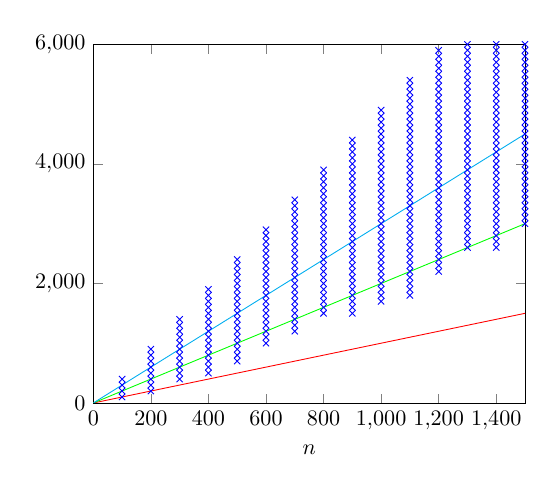
\begin{tikzpicture}[scale=0.8]
		\begin{axis}[
		compat=newest,
		xmin=0,
		xmax=1500,
		ymin=0,
		ymax=6000,
		xlabel={$n$}
		]
		\addplot[
		scatter,only marks,scatter src=explicit symbolic,
		scatter/classes={
			a={mark=x,blue}
		}
		]
		table[x=x,y=y,meta=label]{
			x    y    label
			100  100 a
			100  200 a
			100  300 a
			100  400 a
			200  200 a
			200  300 a
			200  400 a
			200  500 a
			200  600 a
			200  700 a
			200  800 a
			200  900 a
			300  400 a
			300  500 a
			300  600 a
			300  700 a
			300  800 a
			300  900 a
			300  1000 a
			300  1100 a
			300  1200 a
			300  1300 a
			300  1400 a
			400  500 a
			400  600 a
			400  700 a
			400  800 a
			400  900 a
			400  1000 a
			400  1100 a
			400  1200 a
			400  1300 a
			400  1400 a
			400  1500 a
			400  1600 a
			400  1700 a
			400  1800 a
			400  1900 a
			500  700 a
			500  800 a
			500  900 a
			500  1000 a
			500  1100 a
			500  1200 a
			500  1300 a
			500  1400 a
			500  1500 a
			500  1600 a
			500  1700 a
			500  1800 a
			500  1900 a
			500  2000 a
			500  2100 a
			500  2200 a
			500  2300 a
			500  2400 a
			600  1000 a
			600  1100 a
			600  1200 a
			600  1300 a
			600  1400 a
			600  1500 a
			600  1600 a
			600  1700 a
			600  1800 a
			600  1900 a
			600  2000 a
			600  2100 a
			600  2200 a
			600  2300 a
			600  2400 a
			600  2500 a
			600  2600 a
			600  2700 a
			600  2800 a
			600  2900 a
			700  1200 a
			700  1300 a
			700  1400 a
			700  1500 a
			700  1600 a
			700  1700 a
			700  1800 a
			700  1900 a
			700  2000 a
			700  2100 a
			700  2200 a
			700  2300 a
			700  2400 a
			700  2500 a
			700  2600 a
			700  2700 a
			700  2800 a
			700  2900 a
			700  3000 a
			700  3100 a
			700  3200 a
			700  3300 a
			700  3400 a
			800  1500 a
			800  1600 a
			800  1700 a
			800  1800 a
			800  1900 a
			800  2000 a
			800  2100 a
			800  2200 a
			800  2300 a
			800  2400 a
			800  2500 a
			800  2600 a
			800  2700 a
			800  2800 a
			800  2900 a
			800  3000 a
			800  3100 a
			800  3200 a
			800  3300 a
			800  3400 a
			800  3500 a
			800  3600 a
			800  3700 a
			800  3800 a
			800  3900 a
			900  1500 a
			900  1600 a
			900  1700 a
			900  1800 a
			900  1900 a
			900  2000 a
			900  2100 a
			900  2200 a
			900  2300 a
			900  2400 a
			900  2500 a
			900  2600 a
			900  2700 a
			900  2800 a
			900  2900 a
			900  3000 a
			900  3100 a
			900  3200 a
			900  3300 a
			900  3400 a
			900  3500 a
			900  3600 a
			900  3700 a
			900  3800 a
			900  3900 a
			900  4000 a
			900  4100 a
			900  4200 a
			900  4300 a
			900  4400 a
			1000  1700 a
			1000  1800 a
			1000  1900 a
			1000  2000 a
			1000  2100 a
			1000  2200 a
			1000  2300 a
			1000  2400 a
			1000  2500 a
			1000  2600 a
			1000  2700 a
			1000  2800 a
			1000  2900 a
			1000  3000 a
			1000  3100 a
			1000  3200 a
			1000  3300 a
			1000  3400 a
			1000  3500 a
			1000  3600 a
			1000  3700 a
			1000  3800 a
			1000  3900 a
			1000  4000 a
			1000  4100 a
			1000  4200 a
			1000  4300 a
			1000  4400 a
			1000  4500 a
			1000  4600 a
			1000  4700 a
			1000  4800 a
			1000  4900 a
			1100  1800 a
			1100  1900 a
			1100  2000 a
			1100  2100 a
			1100  2200 a
			1100  2300 a
			1100  2400 a
			1100  2500 a
			1100  2600 a
			1100  2700 a
			1100  2800 a
			1100  2900 a
			1100  3000 a
			1100  3100 a
			1100  3200 a
			1100  3300 a
			1100  3400 a
			1100  3500 a
			1100  3600 a
			1100  3700 a
			1100  3800 a
			1100  3900 a
			1100  4000 a
			1100  4100 a
			1100  4200 a
			1100  4300 a
			1100  4400 a
			1100  4500 a
			1100  4600 a
			1100  4700 a
			1100  4800 a
			1100  4900 a
			1100  5000 a
			1100  5100 a
			1100  5200 a
			1100  5300 a
			1100  5400 a
			1200  2200 a
			1200  2300 a
			1200  2400 a
			1200  2500 a
			1200  2600 a
			1200  2700 a
			1200  2800 a
			1200  2900 a
			1200  3000 a
			1200  3100 a
			1200  3200 a
			1200  3300 a
			1200  3400 a
			1200  3500 a
			1200  3600 a
			1200  3700 a
			1200  3800 a
			1200  3900 a
			1200  4000 a
			1200  4100 a
			1200  4200 a
			1200  4300 a
			1200  4400 a
			1200  4500 a
			1200  4600 a
			1200  4700 a
			1200  4800 a
			1200  4900 a
			1200  5000 a
			1200  5100 a
			1200  5200 a
			1200  5300 a
			1200  5400 a
			1200  5500 a
			1200  5600 a
			1200  5700 a
			1200  5800 a
			1200  5900 a
			1300  2600 a
			1300  2700 a
			1300  2800 a
			1300  2900 a
			1300  3000 a
			1300  3100 a
			1300  3200 a
			1300  3300 a
			1300  3400 a
			1300  3500 a
			1300  3600 a
			1300  3700 a
			1300  3800 a
			1300  3900 a
			1300  4000 a
			1300  4100 a
			1300  4200 a
			1300  4300 a
			1300  4400 a
			1300  4500 a
			1300  4600 a
			1300  4700 a
			1300  4800 a
			1300  4900 a
			1300  5000 a
			1300  5100 a
			1300  5200 a
			1300  5300 a
			1300  5400 a
			1300  5500 a
			1300  5600 a
			1300  5700 a
			1300  5800 a
			1300  5900 a
			1300  6000 a
			1300  6100 a
			1300  6200 a
			1300  6300 a
			1300  6400 a
			1400  2600 a
			1400  2700 a
			1400  2800 a
			1400  2900 a
			1400  3000 a
			1400  3100 a
			1400  3200 a
			1400  3300 a
			1400  3400 a
			1400  3500 a
			1400  3600 a
			1400  3700 a
			1400  3800 a
			1400  3900 a
			1400  4000 a
			1400  4100 a
			1400  4200 a
			1400  4300 a
			1400  4400 a
			1400  4500 a
			1400  4600 a
			1400  4700 a
			1400  4800 a
			1400  4900 a
			1400  5000 a
			1400  5100 a
			1400  5200 a
			1400  5300 a
			1400  5400 a
			1400  5500 a
			1400  5600 a
			1400  5700 a
			1400  5800 a
			1400  5900 a
			1400  6000 a
			1400  6100 a
			1400  6200 a
			1400  6300 a
			1400  6400 a
			1400  6500 a
			1400  6600 a
			1400  6700 a
			1400  6800 a
			1400  6900 a
			1500  3000 a
			1500  3100 a
			1500  3200 a
			1500  3300 a
			1500  3400 a
			1500  3500 a
			1500  3600 a
			1500  3700 a
			1500  3800 a
			1500  3900 a
			1500  4000 a
			1500  4100 a
			1500  4200 a
			1500  4300 a
			1500  4400 a
			1500  4500 a
			1500  4600 a
			1500  4700 a
			1500  4800 a
			1500  4900 a
			1500  5000 a
			1500  5100 a
			1500  5200 a
			1500  5300 a
			1500  5400 a
			1500  5500 a
			1500  5600 a
			1500  5700 a
			1500  5800 a
			1500  5900 a
			1500  6000 a
			1500  6100 a
			1500  6200 a
			1500  6300 a
			1500  6400 a
			1500  6500 a
			1500  6600 a
			1500  6700 a
			1500  6800 a
			1500  6900 a
			1500  7000 a
			1500  7100 a
			1500  7200 a
			1500  7300 a
			1500  7400 a
			1600  3200 a
			1600  3300 a
			1600  3400 a
			1600  3500 a
			1600  3600 a
			1600  3700 a
			1600  3800 a
			1600  3900 a
			1600  4000 a
			1600  4100 a
			1600  4200 a
			1600  4300 a
			1600  4400 a
			1600  4500 a
			1600  4600 a
			1600  4700 a
			1600  4800 a
			1600  4900 a
			1600  5000 a
			1600  5100 a
			1600  5200 a
			1600  5300 a
			1600  5400 a
			1600  5500 a
			1600  5600 a
			1600  5700 a
			1600  5800 a
			1600  5900 a
			1600  6000 a
			1600  6100 a
			1600  6200 a
			1600  6300 a
			1600  6400 a
			1600  6500 a
			1600  6600 a
			1600  6700 a
			1600  6800 a
			1600  6900 a
			1600  7000 a
			1600  7100 a
			1600  7200 a
			1600  7300 a
			1600  7400 a
			1600  7500 a
			1600  7600 a
			1600  7700 a
			1600  7800 a
			1600  7900 a
			1700  3300 a
			1700  3400 a
			1700  3500 a
			1700  3600 a
			1700  3700 a
			1700  3800 a
			1700  3900 a
			1700  4000 a
			1700  4100 a
			1700  4200 a
			1700  4300 a
			1700  4400 a
			1700  4500 a
			1700  4600 a
			1700  4700 a
			1700  4800 a
			1700  4900 a
			1700  5000 a
			1700  5100 a
			1700  5200 a
			1700  5300 a
			1700  5400 a
			1700  5500 a
			1700  5600 a
			1700  5700 a
			1700  5800 a
			1700  5900 a
			1700  6000 a
			1700  6100 a
			1700  6200 a
			1700  6300 a
			1700  6400 a
			1700  6500 a
			1700  6600 a
			1700  6700 a
			1700  6800 a
			1700  6900 a
			1700  7000 a
			1700  7100 a
			1700  7200 a
			1700  7300 a
			1700  7400 a
			1700  7500 a
			1700  7600 a
			1700  7700 a
			1700  7800 a
			1700  7900 a
			1700  8000 a
			1700  8100 a
			1700  8200 a
			1700  8300 a
			1700  8400 a
			1800  3900 a
			1800  4000 a
			1800  4100 a
			1800  4200 a
			1800  4300 a
			1800  4400 a
			1800  4500 a
			1800  4600 a
			1800  4700 a
			1800  4800 a
			1800  4900 a
			1800  5000 a
			1800  5100 a
			1800  5200 a
			1800  5300 a
			1800  5400 a
			1800  5500 a
			1800  5600 a
			1800  5700 a
			1800  5800 a
			1800  5900 a
			1800  6000 a
			1800  6100 a
			1800  6200 a
			1800  6300 a
			1800  6400 a
			1800  6500 a
			1800  6600 a
			1800  6700 a
			1800  6800 a
			1800  6900 a
			1800  7000 a
			1800  7100 a
			1800  7200 a
			1800  7300 a
			1800  7400 a
			1800  7500 a
			1800  7600 a
			1800  7700 a
			1800  7800 a
			1800  7900 a
			1800  8000 a
			1800  8100 a
			1800  8200 a
			1800  8300 a
			1800  8400 a
			1800  8500 a
			1800  8600 a
			1800  8700 a
			1800  8800 a
			1800  8900 a
			1900  4000 a
			1900  4100 a
			1900  4200 a
			1900  4300 a
			1900  4400 a
			1900  4500 a
			1900  4600 a
			1900  4700 a
			1900  4800 a
			1900  4900 a
			1900  5000 a
			1900  5100 a
			1900  5200 a
			1900  5300 a
			1900  5400 a
			1900  5500 a
			1900  5600 a
			1900  5700 a
			1900  5800 a
			1900  5900 a
			1900  6000 a
			1900  6100 a
			1900  6200 a
			1900  6300 a
			1900  6400 a
			1900  6500 a
			1900  6600 a
			1900  6700 a
			1900  6800 a
			1900  6900 a
			1900  7000 a
			1900  7100 a
			1900  7200 a
			1900  7300 a
			1900  7400 a
			1900  7500 a
			1900  7600 a
			1900  7700 a
			1900  7800 a
			1900  7900 a
			1900  8000 a
			1900  8100 a
			1900  8200 a
			1900  8300 a
			1900  8400 a
			1900  8500 a
			1900  8600 a
			1900  8700 a
			1900  8800 a
			1900  8900 a
			1900  9000 a
			1900  9100 a
			1900  9200 a
			1900  9300 a
			1900  9400 a
			2000  2000 a
			2000  2100 a
			2000  2200 a
			2000  2300 a
			2000  2400 a
			2000  2500 a
			2000  2600 a
			2000  2700 a
			2000  2800 a
			2000  2900 a
			2000  3000 a
			2000  3100 a
			2000  3200 a
			2000  3300 a
			2000  3400 a
			2000  3500 a
			2000  3600 a
			2000  3700 a
			2000  3800 a
			2000  3900 a
			2000  4000 a
			2000  4100 a
			2000  4200 a
			2000  4300 a
			2000  4400 a
			2000  4500 a
			2000  4600 a
			2000  4700 a
			2000  4800 a
			2000  4900 a
			2000  5000 a
			2000  5100 a
			2000  5200 a
			2000  5300 a
			2000  5400 a
			2000  5500 a
			2000  5600 a
			2000  5700 a
			2000  5800 a
			2000  5900 a
			2000  6000 a
			2000  6100 a
			2000  6200 a
			2000  6300 a
			2000  6400 a
			2000  6500 a
			2000  6600 a
			2000  6700 a
			2000  6800 a
			2000  6900 a
			2000  7000 a
			2000  7100 a
			2000  7200 a
			2000  7300 a
			2000  7400 a
			2000  7500 a
			2000  7600 a
			2000  7700 a
			2000  7800 a
			2000  7900 a
			2000  8000 a
			2000  8100 a
			2000  8200 a
			2000  8300 a
			2000  8400 a
			2000  8500 a
			2000  8600 a
			2000  8700 a
			2000  8800 a
			2000  8900 a
			2000  9000 a
			2000  9100 a
			2000  9200 a
			2000  9300 a
			2000  9400 a
			2000  9500 a
			2000  9600 a
			2000  9700 a
			2000  9800 a
			2000  9900 a
			2100  4100 a
			2100  4200 a
			2100  4300 a
			2100  4400 a
			2100  4500 a
			2100  4600 a
			2100  4700 a
			2100  4800 a
			2100  4900 a
			2100  5000 a
			2100  5100 a
			2100  5200 a
			2100  5300 a
			2100  5400 a
			2100  5500 a
			2100  5600 a
			2100  5700 a
			2100  5800 a
			2100  5900 a
			2100  6000 a
			2100  6100 a
			2100  6200 a
			2100  6300 a
			2100  6400 a
			2100  6500 a
			2100  6600 a
			2100  6700 a
			2100  6800 a
			2100  6900 a
			2100  7000 a
			2100  7100 a
			2100  7200 a
			2100  7300 a
			2100  7400 a
			2100  7500 a
			2100  7600 a
			2100  7700 a
			2100  7800 a
			2100  7900 a
			2100  8000 a
			2100  8100 a
			2100  8200 a
			2100  8300 a
			2100  8400 a
			2100  8500 a
			2100  8600 a
			2100  8700 a
			2100  8800 a
			2100  8900 a
			2100  9000 a
			2100  9100 a
			2100  9200 a
			2100  9300 a
			2100  9400 a
			2100  9500 a
			2100  9600 a
			2100  9700 a
			2100  9800 a
			2100  9900 a
			2100  10000 a
			2200  4500 a
			2200  4600 a
			2200  4700 a
			2200  4800 a
			2200  4900 a
			2200  5000 a
			2200  5100 a
			2200  5200 a
			2200  5300 a
			2200  5400 a
			2200  5500 a
			2200  5600 a
			2200  5700 a
			2200  5800 a
			2200  5900 a
			2200  6000 a
			2200  6100 a
			2200  6200 a
			2200  6300 a
			2200  6400 a
			2200  6500 a
			2200  6600 a
			2200  6700 a
			2200  6800 a
			2200  6900 a
			2200  7000 a
			2200  7100 a
			2200  7200 a
			2200  7300 a
			2200  7400 a
			2200  7500 a
			2200  7600 a
			2200  7700 a
			2200  7800 a
			2200  7900 a
			2200  8000 a
			2200  8100 a
			2200  8200 a
			2200  8300 a
			2200  8400 a
			2200  8500 a
			2200  8600 a
			2200  8700 a
			2200  8800 a
			2200  8900 a
			2200  9000 a
			2200  9100 a
			2200  9200 a
			2200  9300 a
			2200  9400 a
			2200  9500 a
			2200  9600 a
			2200  9700 a
			2200  9800 a
			2200  9900 a
			2200  10000 a
			2300  4900 a
			2300  5000 a
			2300  5100 a
			2300  5200 a
			2300  5300 a
			2300  5400 a
			2300  5500 a
			2300  5600 a
			2300  5700 a
			2300  5800 a
			2300  5900 a
			2300  6000 a
			2300  6100 a
			2300  6200 a
			2300  6300 a
			2300  6400 a
			2300  6500 a
			2300  6600 a
			2300  6700 a
			2300  6800 a
			2300  6900 a
			2300  7000 a
			2300  7100 a
			2300  7200 a
			2300  7300 a
			2300  7400 a
			2300  7500 a
			2300  7600 a
			2300  7700 a
			2300  7800 a
			2300  7900 a
			2300  8000 a
			2300  8100 a
			2300  8200 a
			2300  8300 a
			2300  8400 a
			2300  8500 a
			2300  8600 a
			2300  8700 a
			2300  8800 a
			2300  8900 a
			2300  9000 a
			2300  9100 a
			2300  9200 a
			2300  9300 a
			2300  9400 a
			2300  9500 a
			2300  9600 a
			2300  9700 a
			2300  9800 a
			2300  9900 a
			2300  10000 a
			2400  5200 a
			2400  5300 a
			2400  5400 a
			2400  5500 a
			2400  5600 a
			2400  5700 a
			2400  5800 a
			2400  5900 a
			2400  6000 a
			2400  6100 a
			2400  6200 a
			2400  6300 a
			2400  6400 a
			2400  6500 a
			2400  6600 a
			2400  6700 a
			2400  6800 a
			2400  6900 a
			2400  7000 a
			2400  7100 a
			2400  7200 a
			2400  7300 a
			2400  7400 a
			2400  7500 a
			2400  7600 a
			2400  7700 a
			2400  7800 a
			2400  7900 a
			2400  8000 a
			2400  8100 a
			2400  8200 a
			2400  8300 a
			2400  8400 a
			2400  8500 a
			2400  8600 a
			2400  8700 a
			2400  8800 a
			2400  8900 a
			2400  9000 a
			2400  9100 a
			2400  9200 a
			2400  9300 a
			2400  9400 a
			2400  9500 a
			2400  9600 a
			2400  9700 a
			2400  9800 a
			2400  9900 a
			2400  10000 a
		};
		\draw[color=red] (0,0) -- (1500,1500) node[right] {a};
		\draw[color=green] (0,0) -- (1500,3000);
		\draw[color=cyan] (0,0) -- (1500,4500);
		\end{axis}
	  \end{tikzpicture}
	  \caption{Uniquely satisfiable instances found.}{Red: $n=m$; Green: $2n=m$; Cyan:$3n=m$; Crosses: Uniquely satisfiable instances found}
	  \label{fig:inst}
	  
\end{figure}
\newpage
\subsection{Performance}
Here we present the performance of varying packages. Figure \ref{fig:px} displays the timings of the three packages created. Figure \ref{fig:py} illustrates our most difficult package \emph{con\_sml} versus existing benchmarks. Results showed that we consistently produced graphs which executed for longer than three hours, however, since many of the packages did not execute for longer than the specified timeout, we could not compare graphs of equal sizes for most graphs which timed out. 


\begin{figure}[htbp!] 
	\centering
	\begin{minipage}{.4\textwidth}
		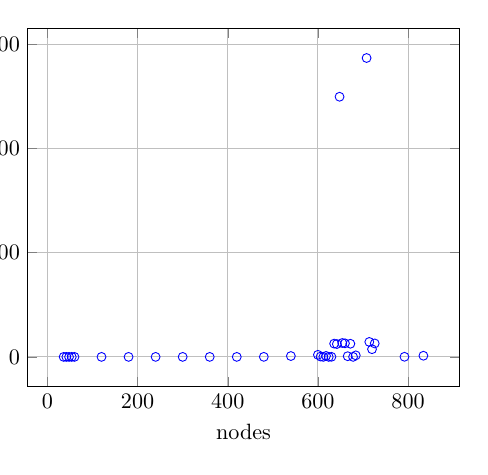
\begin{tikzpicture}[trim left=0cm, scale=0.8]
		\begin{axis}[
		xlabel=nodes,
		ylabel=t sec,
		grid=both,
		]
		\addplot[
		scatter,only marks,scatter src=explicit symbolic,
		scatter/classes={
			a={mark=o,blue}
		}
		]
		table[x=x,y=y,meta=label]{
			x    y    label
			36	0.000504970550537	a
			42	0.000595092773438	a
			48	0.000430107116699	a
			54	0.000416994094849	a
			60	0.000868082046509	a
			120	0.0010769367218	a
			180	0.00196194648743	a
			240	0.0024151802063	a
			300	0.00288486480713	a
			360	0.00310897827148	a
			420	0.00304412841797	a
			480	0.0377099514008	a
			540	0.822341918945	a
			600	1.99121904373	a
			606	0.287495136261	a
			612	0.0140619277954	a
			618	0.919209003448	a
			624	0.014004945755	a
			630	0.0803589820862	a
			636	12.7223041058	a
			642	12.3259220123	a
			648	249.624564171	a
			654	13.3357129097	a
			660	13.0116429329	a
			666	0.671919822693	a
			672	12.6001150608	a
			678	0.0159549713135	a
			684	1.46877002716	a
			708	286.804507017	a
			714	14.3620049953	a
			720	7.38974690437	a
			726	12.9122009277	a
			792	0.103566884995	a
			834	1.10935306549	a
		};
		\end{axis}
		\end{tikzpicture}
		
	\end{minipage}
	\begin{minipage}{.4\textwidth}
		\centering
		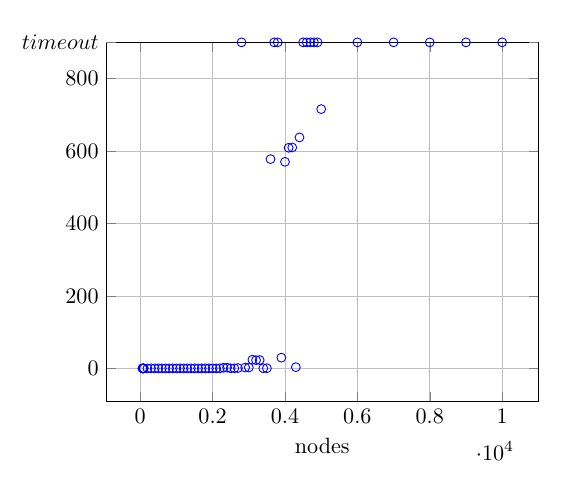
\begin{tikzpicture}[trim left=-1cm, scale=0.8]
		\begin{axis}[
		xlabel=nodes,
		ylabel=t sec,
		grid=both,
		extra y ticks={900},
		extra y tick labels={\hspace{5em}$timeout$},
		extra y tick style={grid=none},
		ymax=900,
		]
		\addplot[
		scatter,only marks,scatter src=explicit symbolic,
		scatter/classes={
			a={mark=o,blue}
		}
		]
		table[x=x,y=y,meta=label]{
			x    y    label
			60	0.00088095664978	a
			70	0.000917196273804	a
			80	0.000850915908813	a
			90	0.000887870788574	a
			100	0.000802040100098	a
			200	0.000893115997314	a
			300	0.00113701820374	a
			400	0.00194406509399	a
			500	0.00256896018982	a
			600	0.00155901908875	a
			700	0.00173497200012	a
			800	0.00396299362183	a
			900	0.00400900840759	a
			1000	0.00220799446106	a
			1100	0.0236101150513	a
			1200	0.00546789169312	a
			1300	0.00626587867737	a
			1400	0.00990104675293	a
			1500	0.0394530296326	a
			1600	0.0112538337708	a
			1700	0.0123739242554	a
			1800	0.0139899253845	a
			1900	0.0278260707855	a
			2000	0.0534319877625	a
			2100	0.00984311103821	a
			2200	0.0178880691528	a
			2300	1.90173387527	a
			2400	2.04471302032	a
			2500	0.200901985168	a
			2600	0.327310085297	a
			2700	0.923086881638	a
			2800	900	a
			2900	2.30818605423	a
			3000	2.48632717133	a
			3100	23.9029829502	a
			3200	22.727894783	a
			3300	23.0080840588	a
			3400	0.441438913345	a
			3500	0.49547791481	a
			3600	577.676494122	a
			3700	900	a
			3800	900	a
			3900	29.6461250782	a
			4000	570.171611071	a
			4100	609.037957907	a
			4200	609.872159004	a
			4300	3.48693990707	a
			4400	637.644945145	a
			4500	900	a
			4600	900	a
			4700	900	a
			4800	900	a
			4900	900	a
			5000	715.732777119	a
			6000	900	a
			7000	900	a
			8000	900	a
			9000	900	a
			10000	900	a
		};
		\end{axis}
		\end{tikzpicture}
	\end{minipage}
	\\	
	\begin{minipage}{.4\textwidth}	
		\centering
		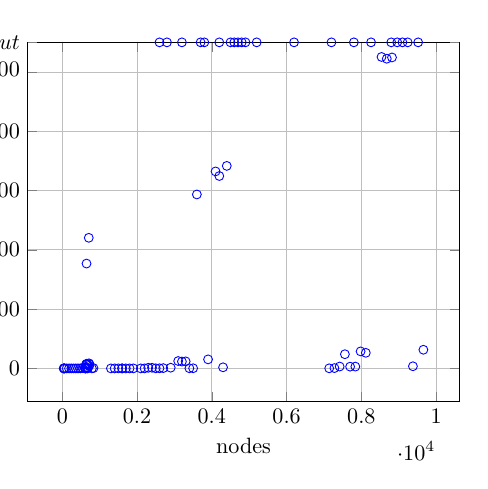
\begin{tikzpicture}[trim left=0cm, scale=0.8]
		\begin{axis}[
		xlabel=nodes,
		ylabel=t sec,
		grid=both,
		extra y ticks={1100},
		extra tick style={grid=major, grid style={dotted, cyan}},
		extra y tick labels={\hspace{5em}$timeout$},
		extra x tick labels={},
		extra y tick style={grid=none},
		ymax=1100
		]
		\addplot[
		scatter,only marks,scatter src=explicit symbolic,
		scatter/classes={
			a={mark=o,blue}
		}
		]
		table[x=x,y=y,meta=label]{
			x    y    label
			36	0.00103306770325	a
			42	0.000981092453003	a
			48	0.000943899154663	a
			54	0.000932931900024	a
			60	0.000885009765625	a
			120	0.00100302696228	a
			180	0.00216317176819	a
			240	0.0023980140686	a
			300	0.00391316413879	a
			360	0.00308299064636	a
			420	0.00360012054443	a
			480	0.0388169288635	a
			540	0.885004997253	a
			600	2.20803809166	a
			606	0.286993980408	a
			612	0.0141770839691	a
			618	1.02969312668	a
			624	0.0157458782196	a
			630	0.0813388824463	a
			636	13.5863618851	a
			642	13.4802289009	a
			648	353.685708046	a
			654	15.9124789238	a
			660	0.967444896698	a
			666	0.688606977463	a
			672	14.1916108131	a
			678	0.0158090591431	a
			684	1.52013897896	a
			708	440.586826086	a
			714	17.1741900444	a
			720	8.75624012947	a
			726	14.2599079609	a
			1300	0.00624203681946	a
			792	0.0990188121796	a
			834	1.13995695114	a
			1400	0.0105519294739	a
			1500	0.0400409698486	a
			1600	0.0119650363922	a
			1700	0.0137841701508	a
			1800	0.0135757923126	a
			1900	0.0268559455872	a
			1600	0.189525842667	a
			2100	0.0101490020752	a
			2200	0.0251288414001	a
			2300	2.07047104836	a
			2400	2.17357993126	a
			2500	0.224191904068	a
			2600	0.327886104584	a
			2700	0.934176206589	a
			2800	1100	a
			2900	2.35056710243	a
			2600	1100	a
			3100	24.9071788788	a
			3200	23.0961768627	a
			3300	23.7306361198	a
			3400	0.444133996964	a
			3500	0.506667852402	a
			3600	586.845415115	a
			3700	1100	a
			3800	1100	a
			3900	30.4615390301	a
			3200	1100	a
			4100	664.525188208	a
			4200	649.032501936	a
			4300	3.69031596184	a
			4400	683.195003986	a
			4500	1100	a
			4600	1100	a
			4700	1100	a
			4800	1100	a
			4900	1100	a
			4200	1100	a
			7140	0.266206026077	a
			7280	1.01169610023	a
			7420	6.30038094521	a
			7560	47.8593740463	a
			7700	5.88605880737	a
			7840	6.14195013046	a
			7980	57.4095039368	a
			8120	52.5715360641	a
			8260	1100	a
			5200	1100	a
			8540	1050.74244285	a
			8680	1044.69068694	a
			8820	1049.08241892	a
			8960	1100	a
			9100	1100	a
			9240	1100	a
			9380	7.24794602394	a
			9520	1100	a
			9660	62.879360199	a
			6200	1100	a
			7200	1100	a
			7800	1100	a
			8800	1100	a
		};
		\end{axis}
		\end{tikzpicture}
	\end{minipage}
	\captionsetup{justification=centering}
	\caption{Left: n=m (con\_n).\\
		Right: n=2m (con\_2n). \\
		Center: smallest ratios found (con\_sml)}
	\label{fig:px}
\end{figure}
\begin{figure}[htbp!]
	\centering
	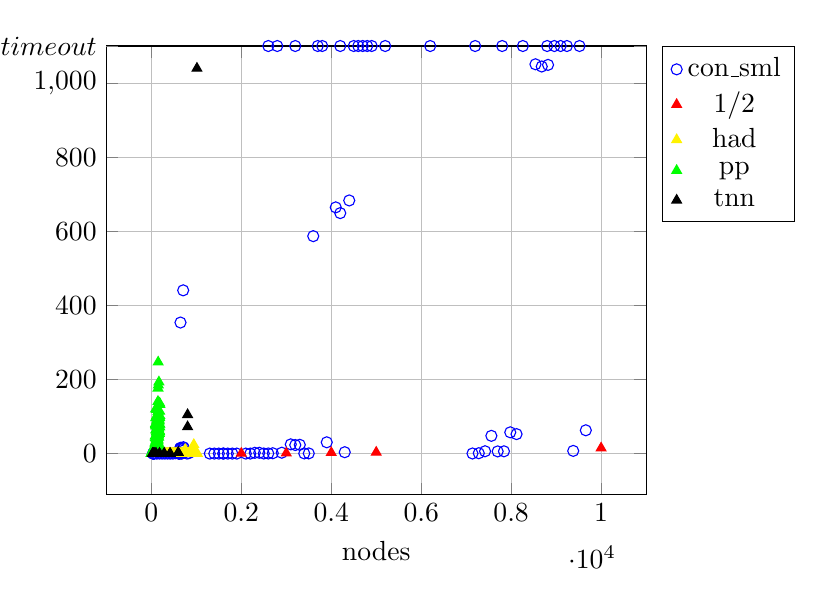
\begin{tikzpicture}[trim left = -1cm, scale=1]
	\begin{axis}[
	xlabel=nodes,
	ylabel=t sec,
	grid=both,
	extra y ticks={1100},
	extra tick style={grid=major, grid style={dotted, cyan}},
	extra y tick labels={\hspace{5em}$timeout$},
	extra x tick labels={},
	extra y tick style={grid=none},
	legend pos=outer north east,
	ymax=1100
	]
	\legend{con\_sml, 1/2, had, pp, tnn}
	\addplot[
	scatter,only marks,scatter src=explicit symbolic,
	scatter/classes={
		a={mark=o,blue},
		b={mark=triangle*,red},
		c={mark=triangle*,yellow},
		d={mark=triangle*,green},
		e={mark=triangle*,black}
	}
	]
	table[x=x,y=y,meta=label]{
		x    y    label
		36	0.00103306770325	a
		42	0.000981092453003	a
		48	0.000943899154663	a
		54	0.000932931900024	a
		60	0.000885009765625	a
		120	0.00100302696228	a
		180	0.00216317176819	a
		240	0.0023980140686	a
		300	0.00391316413879	a
		360	0.00308299064636	a
		420	0.00360012054443	a
		480	0.0388169288635	a
		540	0.885004997253	a
		600	2.20803809166	a
		606	0.286993980408	a
		612	0.0141770839691	a
		618	1.02969312668	a
		624	0.0157458782196	a
		630	0.0813388824463	a
		636	13.5863618851	a
		642	13.4802289009	a
		648	353.685708046	a
		654	15.9124789238	a
		660	0.967444896698	a
		666	0.688606977463	a
		672	14.1916108131	a
		678	0.0158090591431	a
		684	1.52013897896	a
		708	440.586826086	a
		714	17.1741900444	a
		720	8.75624012947	a
		726	14.2599079609	a
		1300	0.00624203681946	a
		792	0.0990188121796	a
		834	1.13995695114	a
		1400	0.0105519294739	a
		1500	0.0400409698486	a
		1600	0.0119650363922	a
		1700	0.0137841701508	a
		1800	0.0135757923126	a
		1900	0.0268559455872	a
		1600	0.189525842667	a
		2100	0.0101490020752	a
		2200	0.0251288414001	a
		2300	2.07047104836	a
		2400	2.17357993126	a
		2500	0.224191904068	a
		2600	0.327886104584	a
		2700	0.934176206589	a
		2800	1100	a
		2900	2.35056710243	a
		2600	1100	a
		3100	24.9071788788	a
		3200	23.0961768627	a
		3300	23.7306361198	a
		3400	0.444133996964	a
		3500	0.506667852402	a
		3600	586.845415115	a
		3700	1100	a
		3800	1100	a
		3900	30.4615390301	a
		3200	1100	a
		4100	664.525188208	a
		4200	649.032501936	a
		4300	3.69031596184	a
		4400	683.195003986	a
		4500	1100	a
		4600	1100	a
		4700	1100	a
		4800	1100	a
		4900	1100	a
		4200	1100	a
		7140	0.266206026077	a
		7280	1.01169610023	a
		7420	6.30038094521	a
		7560	47.8593740463	a
		7700	5.88605880737	a
		7840	6.14195013046	a
		7980	57.4095039368	a
		8120	52.5715360641	a
		8260	1100	a
		5200	1100	a
		8540	1050.74244285	a
		8680	1044.69068694	a
		8820	1049.08241892	a
		8960	1100	a
		9100	1100	a
		9240	1100	a
		9380	7.24794602394	a
		9520	1100	a
		9660	62.879360199	a
		6200	1100	a
		7200	1100	a
		7800	1100	a
		8800	1100	a
		5	0.000801086425781	b
		10	0.000857830047607	b
		15	0.000815868377686	b
		20	0.00086498260498	b
		25	0.000833034515381	b
		30	0.000885009765625	b
		40	0.00108909606934	b
		50	0.000993013381958	b
		60	0.00110292434692	b
		70	0.00121307373047	b
		80	0.0013689994812	b
		100	0.00164794921875	b
		200	0.00490808486938	b
		300	0.0093150138855	b
		400	0.0167360305786	b
		500	0.0253059864044	b
		600	0.057608127594	b
		700	0.0520691871643	b
		800	0.0675909519196	b
		900	0.0881798267365	b
		1000	0.10640001297	b
		2000	0.486861944199	b
		3000	1.15394091606	b
		4000	2.44690203667	b
		5000	3.31565213203	b
		10000	14.8829817772	b
		4	0.000930070877075	c
		8	0.000865936279297	c
		16	0.000845193862915	c
		32	0.000930786132812	c
		48	0.00147294998169	c
		64	0.00136494636536	c
		80	0.00255489349365	c
		96	0.00285792350769	c
		112	0.00303387641907	c
		128	0.00530004501343	c
		144	0.00288701057434	c
		160	0.00666308403015	c
		176	0.00345611572266	c
		192	0.00493788719177	c
		208	0.0167338848114	c
		224	0.0145990848541	c
		240	0.00622987747192	c
		256	0.00490307807922	c
		272	0.00505113601685	c
		288	0.00681591033936	c
		304	0.00606393814087	c
		320	0.0118939876556	c
		336	0.0076220035553	c
		352	0.0107100009918	c
		368	0.1057908535	c
		384	0.0120139122009	c
		400	0.0673158168793	c
		416	0.0125169754028	c
		432	0.0138850212097	c
		448	0.0296130180359	c
		464	0.093101978302	c
		480	0.0204088687897	c
		496	0.0136818885803	c
		512	0.0128610134125	c
		528	0.017657995224	c
		544	0.0184848308563	c
		560	0.0129160881042	c
		576	0.0185670852661	c
		592	0.0293200016022	c
		608	0.0233659744263	c
		624	0.253060817719	c
		640	0.0492939949036	c
		656	0.0243890285492	c
		672	0.0193901062012	c
		688	0.183281898499	c
		704	0.194499969482	c
		720	0.0207889080048	c
		736	0.749053001404	c
		752	10.9565410614	c
		768	0.0408179759979	c
		784	0.0409290790558	c
		800	0.029314994812	c
		816	0.0302150249481	c
		832	0.811336994171	c
		848	0.0284330844879	c
		864	0.0446970462799	c
		880	0.0330929756165	c
		896	0.0468261241913	c
		912	0.0451979637146	c
		928	1.04390501976	c
		944	24.0905220509	c
		960	0.0360689163208	c
		976	0.116590023041	c
		992	0.0725729465485	c
		1008	0.0731618404388	c
		1024	0.0454850196838	c
		1	0.0126891136169	d
		2	0.506518125534	d
		3	0.392946004868	d
		4	0.894825935364	d
		5	0.196982145309	d
		6	0.315265893936	d
		7	0.332309007645	d
		8	0.24335193634	d
		9	0.365062952042	d
		10	1.23158407211	d
		11	1.57859182358	d
		12	1.39838004112	d
		13	5.08932209015	d
		14	0.509947776794	d
		15	0.502409934998	d
		16	2.62835597992	d
		17	1.43174910545	d
		18	1.66480398178	d
		19	1.67586994171	d
		20	0.863186120987	d
		21	0.319430112839	d
		22	1.08262300491	d
		23	0.651422977448	d
		24	2.7789580822	d
		25	2.71859312057	d
		26	1.33379912376	d
		27	1.57668685913	d
		28	0.861810922623	d
		29	0.814624786377	d
		30	0.491320848465	d
		31	0.250020027161	d
		32	0.979526042938	d
		33	0.990874052048	d
		34	1.03750896454	d
		35	1.27122998238	d
		36	1.9730348587	d
		37	1.21517491341	d
		38	2.7824409008	d
		39	4.03445410728	d
		40	2.57081913948	d
		41	0.918713092804	d
		42	9.09311699867	d
		43	4.21852302551	d
		44	2.79935503006	d
		45	1.44041419029	d
		46	13.6960690022	d
		47	4.36718392372	d
		48	5.09262704849	d
		49	6.74439191818	d
		50	0.615566968918	d
		51	1.09924292564	d
		52	0.72227191925	d
		53	2.66123700142	d
		54	10.8986420631	d
		55	2.99331498146	d
		56	2.17653799057	d
		57	4.99392914772	d
		58	0.269629955292	d
		59	8.45138192177	d
		60	7.03433990479	d
		61	4.83216118813	d
		62	14.0986180305	d
		63	7.55382990837	d
		64	5.27514886856	d
		65	5.73121118546	d
		66	8.84520196915	d
		67	16.8682918549	d
		68	0.821696996689	d
		69	3.25065207481	d
		70	19.8054749966	d
		71	7.05913996696	d
		72	9.04616904259	d
		73	16.4374980927	d
		74	14.0369989872	d
		75	18.596724987	d
		76	19.6481587887	d
		77	4.02276992798	d
		78	6.64521002769	d
		79	8.28684687614	d
		80	6.80820798874	d
		81	10.4670460224	d
		82	15.8501479626	d
		83	20.3741481304	d
		84	27.618694067	d
		85	24.964400053	d
		86	46.9837210178	d
		87	19.1491539478	d
		88	20.89427495	d
		89	21.9608399868	d
		90	43.1752519608	d
		91	30.0575361252	d
		92	20.4183228016	d
		93	23.412883997	d
		94	80.7262451649	d
		95	78.2650489807	d
		96	120.296578169	d
		97	74.3564841747	d
		98	96.4089720249	d
		99	63.7082958221	d
		100	12.1158969402	d
		101	4.52894186974	d
		102	18.5163187981	d
		103	13.0482230186	d
		104	27.6333100796	d
		105	29.2300360203	d
		106	34.0243089199	d
		107	35.8039569855	d
		108	41.2593259811	d
		109	25.9144899845	d
		110	39.5159361362	d
		111	20.2451028824	d
		112	76.5514740944	d
		113	58.6134080887	d
		114	47.0111908913	d
		115	77.9892430305	d
		116	59.3557500839	d
		117	101.617552996	d
		118	81.1093401909	d
		119	65.4591360092	d
		120	89.5387251377	d
		121	55.5878548622	d
		122	119.133154154	d
		123	81.5896930695	d
		124	1.21177482605	d
		125	1.75107908249	d
		126	3.16632509232	d
		127	5.85905790329	d
		128	13.6343200207	d
		129	11.5833981037	d
		130	60.361068964	d
		131	16.8550169468	d
		132	19.9720609188	d
		133	14.6795189381	d
		134	18.4900779724	d
		135	60.4171149731	d
		136	21.2625060081	d
		137	16.3078711033	d
		138	73.2241489887	d
		139	37.4852869511	d
		140	39.396668911	d
		141	37.9996068478	d
		142	72.8519239426	d
		143	42.8854019642	d
		144	33.5778288841	d
		145	34.6762301922	d
		146	112.730048895	d
		147	140.33611393	d
		148	176.509591818	d
		149	80.7491970062	d
		150	94.6595630646	d
		151	49.6790251732	d
		152	246.82178092	d
		153	69.8646960258	d
		154	51.3075819016	d
		155	70.2098720074	d
		156	184.636925936	d
		157	49.6054208279	d
		158	101.324445009	d
		159	57.6079769135	d
		160	67.4897480011	d
		161	58.8694310188	d
		162	44.0615730286	d
		163	75.0678899288	d
		164	92.0624268055	d
		165	79.7877941132	d
		166	89.2363080978	d
		167	93.4773800373	d
		168	193.113031864	d
		169	79.252243042	d
		170	55.3960778713	d
		171	54.9066729546	d
		172	101.057892084	d
		173	87.735656023	d
		174	79.8475270271	d
		175	54.1665978432	d
		176	97.7655980587	d
		177	61.4682059288	d
		178	8.47392106056	d
		179	13.4529950619	d
		180	21.0682308674	d
		181	18.5667409897	d
		182	97.3982541561	d
		183	58.7448019981	d
		184	136.06845212	d
		185	71.8858149052	d
		186	113.916485071	d
		187	102.455598116	d
		188	132.602149963	d
		189	78.8722600937	d
		190	11.6795489788	d
		191	21.0182368755	d
		192	3.02556014061	d
		193	7.06277894974	d
		26	0.000897169113159	e
		26	0.000981092453003	e
		52	0.0010359287262	e
		52	0.00107097625732	e
		78	0.00181889533997	e
		78	0.00164103507996	e
		104	0.00313401222229	e
		104	0.00259685516357	e
		182	0.0143599510193	e
		182	0.0137579441071	e
		286	0.0655310153961	e
		286	0.0696680545807	e
		416	0.350058078766	e
		416	0.397336959839	e
		598	2.66647791862	e
		598	2.50128698349	e
		806	72.1839659214	e
		806	104.950797796	e
		1014	1039.76025891	e
		1014	5536.82137489	e
	};
	\end{axis}
	\end{tikzpicture}
	\captionsetup{justification=centering}
	\caption{con\_sml (slowest running graphs) versus benchmarks}
	\label{fig:py}
\end{figure}

\newpage
\section{Discussion}

\subsection{Searching}
Randomly generating our construction given $n$ and $m$ permits us to try and generate many instances of the combinations of $n$ and $m$. So, for any value of $n$ and $m$, we are able to search for instances that lie along the $2n=m$ line. This is better described in the following plot below:

\begin{figure}[h] 
	\centering
	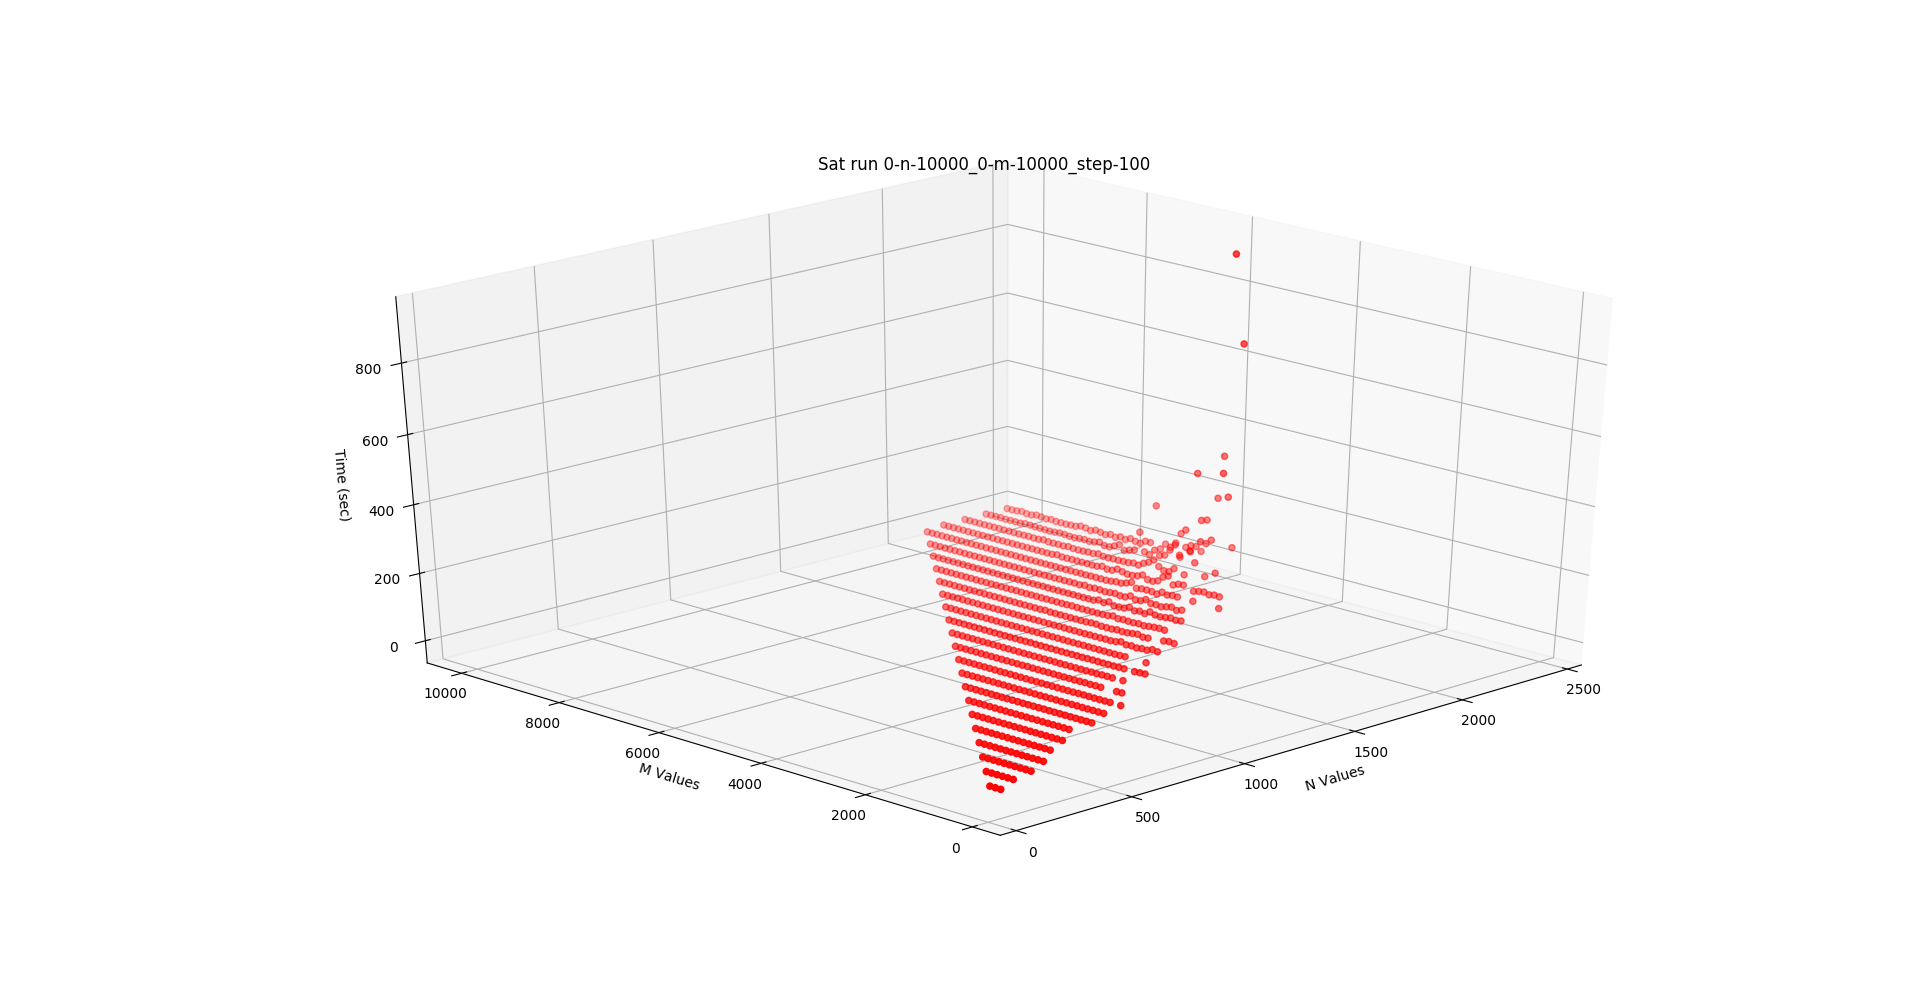
\includegraphics[height=75mm]{Figs/system_search_time}
	\caption{Time taken to search for uniquely satisfiable instances}
	\label{fig:sa}
\end{figure}

(Note that many graphical representations have rendered values illegible. To this end, we will describe some verbally, but retain enlarged images in our package. Such results were not saved as values, but kept as images after long running experiments.)

The $x$ axis represents variables $n$, $y$ represents clauses $m$ and the $z$ axis represents time taken to locate in seconds. This figure was produced after recording the time taken to find a uniquely satisfiable system of equations for combinations of $n$ and $m$. Hence, what we mean by the $2n=m$ line, are those instances which satisfy that equation (e.g. $n=10$ and $m=20$). This is an important distinction ot make, as we see that instances along certain lines differ in time taken to find, namely, those that are rightmost, that is, close to the threshold of satisfiability $n=m$ (the left is bounded by $3n=m$). Figure \ref{fig:sa} shows the cumulative time taken to locate each instance, which means each point includes failures and regenerating and testing instances for unique satisfiability (not necessarily $k$-locally consistent). It does not describe the validation time by Cryptominisat for a single instance, but does hint at this. Figure \ref{fig:sb} illustrates that we have to try much harder near the line of satisfiability to generate uniquely satisfiable systems, shown by the increase in time to the right. We see that for a single instance to be located, it took more than a hour to find a suitable instances near the $n=2000$ and $m=6000$ mark. One point to make, is that the number of tries stays the same. The empty space above lines $n=m$ and below the rightmost plots are instances which were not located using 10 attempts. Hence, it is not only becomes more unlikely to find instances, it also becomes more timely to validate them.

\begin{figure}[htbp!] 
	\centering
	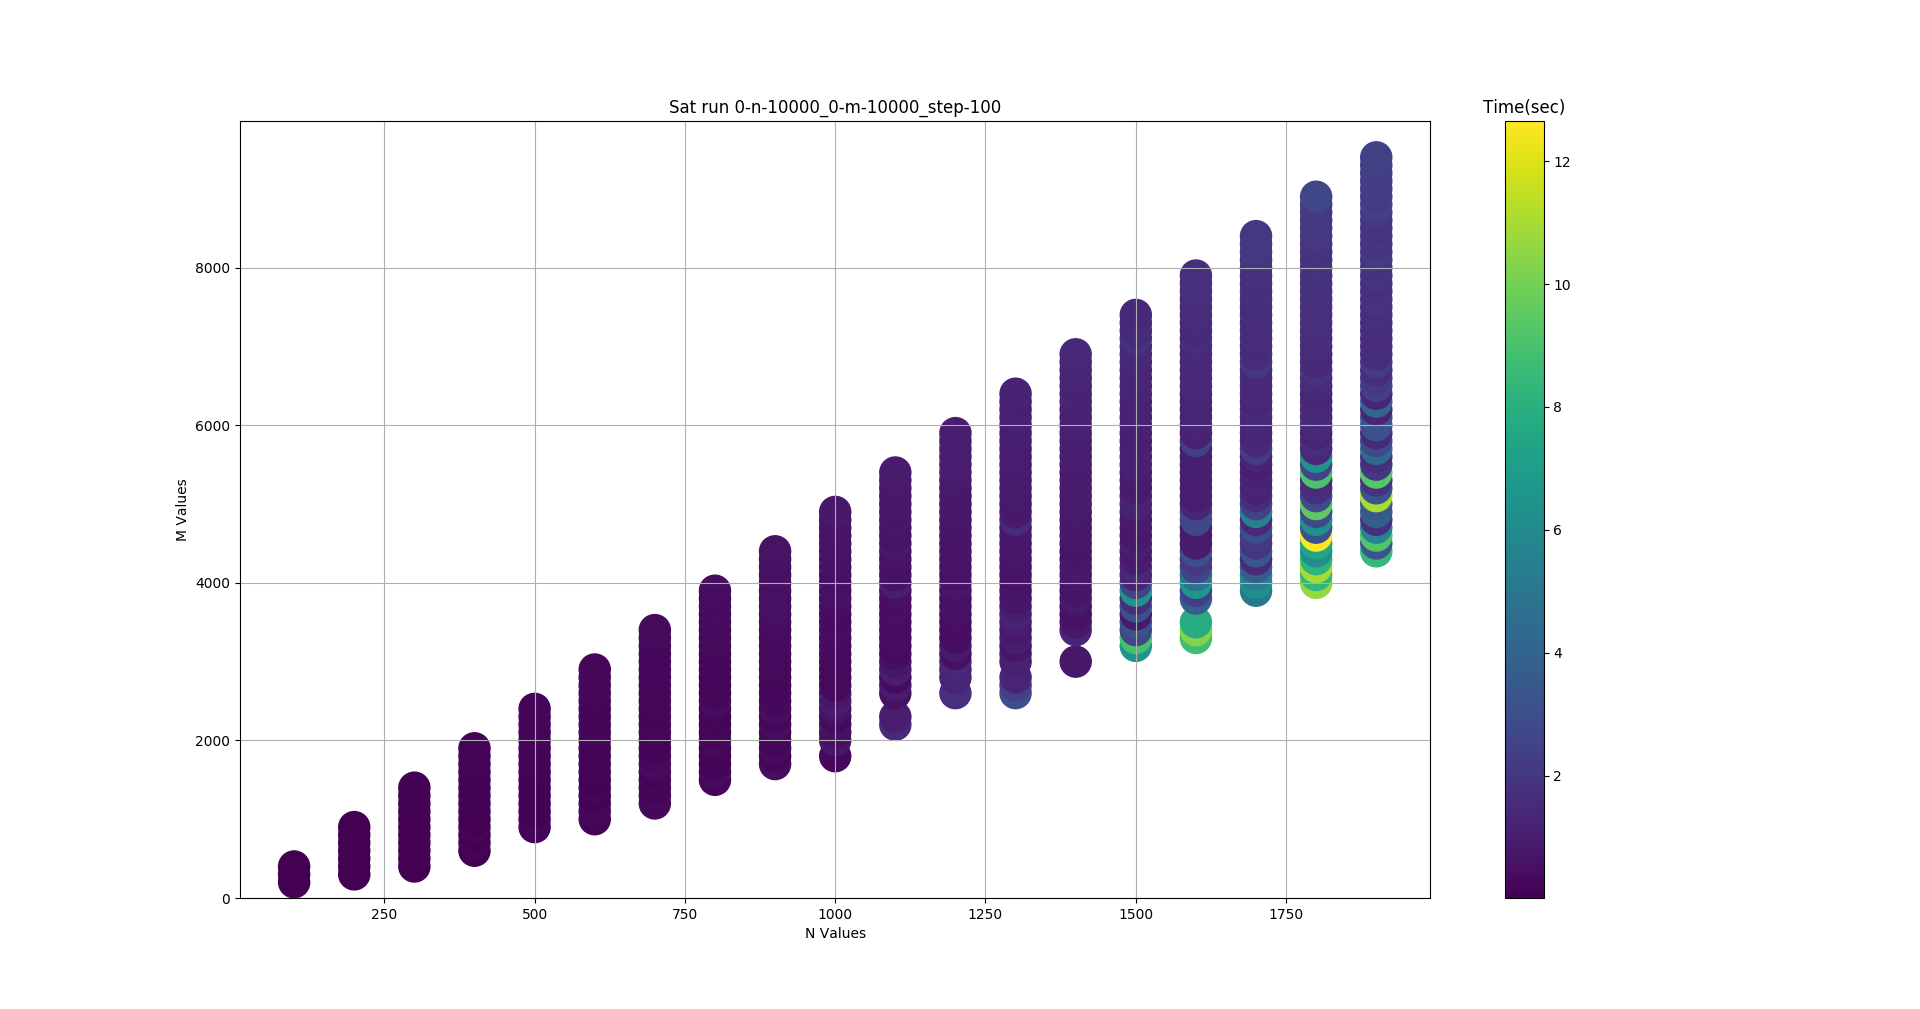
\includegraphics[height=75mm]{Figs/figure_1}
	\caption{Plot of various systems found.}{Note that instances close to the $n=m$ line take far greater time in validation.}
	\label{fig:sb}
\end{figure}

\newpage

\subsection{Validation}
Ensuring we had our desired constructions meant we had to make three checks: $k$-local consistency and unique satisfiability by Cryptominisat, and automorphisms on our preliminary graph using Traces. (Checking for automorphisms is left to Section \ref{sec:aut}.) 

\subsubsection{Unique satisfiability}
Aforementioned, the time taken to check for unique satisfiability increases along the threshold of satisfiability with respect to the size of the systems. Figure \ref{fig:hm} shows this.

\begin{figure}[htbp!] 
	\centering
	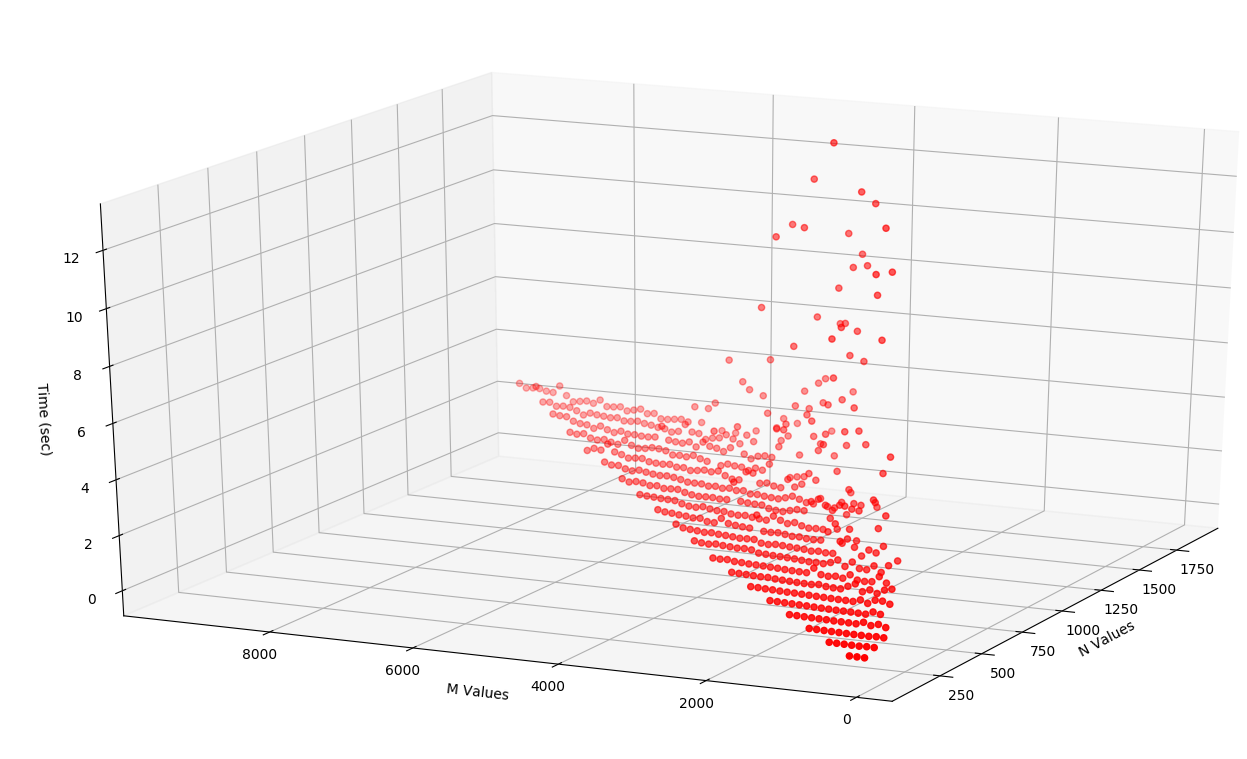
\includegraphics[height=75mm]{Figs/figure_2}
	\caption{Time taken to validate unique satisfiability using Gauss Off}
	\label{fig:hm}
\end{figure}

We note that Cryptominisat works faster with Gauss-Off feature versus Gauss-On. This is Counter-intuitive, since XOR-SAT is known to have a P-Time algorithm using Gaussian elimination. Evidently, validation of unique satisfiability systems, which are along the threshold, appear to take a vastly greater time than those further away. 

\newpage

\subsubsection{$k$-local consistency}
Our makeshift $k$-local consistency check found systems which were significantly quicker using Gauss-On versus Gauss-Off. In our Advanced Search, where we updated our store of slow running systems, that is, with the greatest difference in Gauss-On and Gauss-Off times. The following figure shows systems with negative plots are pseudo k-locally consistent. See Figure \ref{fig:kloc} below.

\begin{figure}[htbp!] 
	\centering
	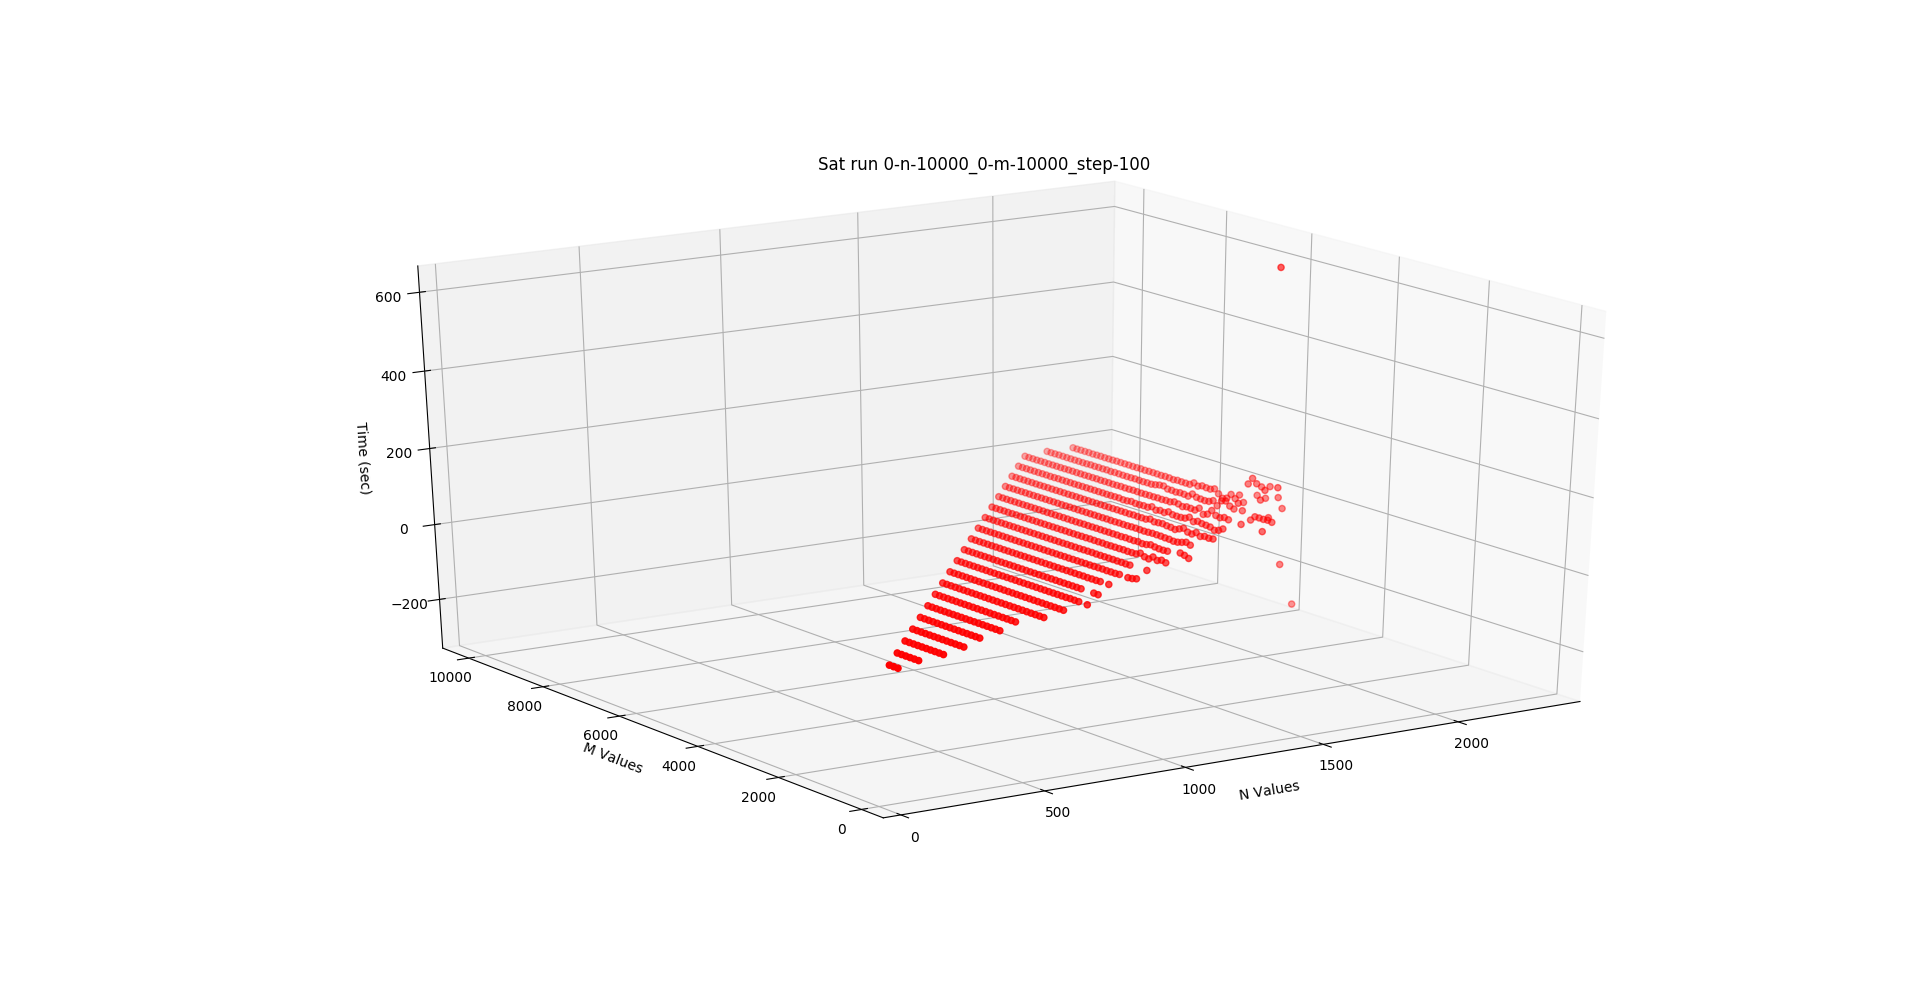
\includegraphics[height=75mm]{Figs/diff_3d}
	\caption{Time taken to validate unique satisfiability Gauss On - Gauss Off.}
	\label{fig:kloc}
\end{figure}

Notice that is more difficult to detect $k$-local consistency the further we move away from the threshold $n=m$. The difference in running times are fairly similar away from $n=m$, but erratic close to $n=m$. Especially as we increase the size of the systems. To which the boundary also moves further away from the line. 

\subsubsection{Strengthening}
As we will prove later, the larger difference between a Gauss-On and Gauss-Off execution time, where Gauss-On is faster for a given uniquely satisfiable 3-XOR-Formula $\phi$, the slower the final graph $G_B$ will be after transforming $\phi$ to $G_B$. Recall that in our Advanced Search we provide the facility to save the slowest found $\phi$. By repeating system searches, and continuously updating the slowest found $\phi$, we filter out very slow systems from the pool of random uniquely satisfiable systems. Hence, repeating a system search 30 times for specific instances, say $n=100$ and $m=100$, we can hope to find a strong instance which is slow for that value of $n$ and $m$. However, it is critical to note that for these values, systems must be readily available and not scarce. 

\newpage

\subsection{Varying Tries}
As we search for instances close to the line of satisfiability $n=m$, our desired construction becomes much more difficult to locate. Recall that the tries parameter in our systems search determines how many times to generate $\phi$ before quitting. 

We noticed that as $n$ and $m$ became larger, if we fixed the number of tries, then it would become more difficult to find instances close to the line of satisfiability. That is to say, as $n$ and $m$ increased, there would be a point where finding $2n=m$ would require more random generations to produce a desired instance, similarly with $3n=m$ and so on. This is better illustrated, but not accurately shown, in Figure \ref{fig:dif} below. The figure depicts that as values of $n$ and $m$ increase, instances along certain lines become scarce. This is important to note, since if we scarcely find instances at certain points, requiring a greater number of tries to locate, we are less likely to filter out a $k$-locally consistent system through repeating runs.

One notable test that can be reproduced is searching along $n=m$, and setting the number of attempts to a large 100,000 attempts to generate a system. One would find that desired instances are hardly available above the $n=m=100$ mark. We know such instances exist, but it becomes increasingly difficult to find an instance for say $n=m=150$. The largest $\phi$ we found for this ratio of $n$ and $m$ is 139, but this was not necessarily $k$-locally consistent as we generated this in 1 run: this is due to scarcely seeing graphs between 105 and 139, that is, many instances exceeded the 100,000 try value. Those below 100 were easy to find (10 tries), and strong systems were found after many iterations, but the same cannot be said for $n>105$, although, this would be ideal since it would produce slow running graphs.

\begin{figure}[h]
	\centering
	\begin{tikzpicture}[trim left=0cm, scale=0.8]
	\begin{axis}[
		xlabel={$n$},
		ylabel=Tries required to locate,
		grid=both,
		extra tick style={grid=major, grid style={dotted, cyan}},
		extra y tick labels={\hspace{5em}$timeout$},
		extra x tick labels={},
		extra y tick style={grid=none},
		yticklabels={,,},
		xticklabels={,,},
		axis lines = left,
		xmin=0,
		clip right=false,
		ymin=0,
		legend pos = north west,
	]
	\addplot[green]  {pow(2,x)};
	\addplot[black]  {pow(2,x-1)};
	\addplot[red]  {pow(2,x-2)};
	\addlegendentry{$n=m$};
	\addlegendentry{$2n=m$};
	\addlegendentry{$3n=m$};
	\end{axis}
	\end{tikzpicture}
	\caption{Illustration of instances becoming scarce}
	\label{fig:dif}
\end{figure}

\newpage
\subsection{Varying Step Size}
In our packages we provide systems and graphs which increase in size by some step factor, as defined in Table \ref{tab:parm}. If we vary the number of steps, we alter the amount of systems produces by our systems search, and ultimately how many graphs are generated. For some packages, for example $con\_n$, we have a step size of 1 between $6<n<10$, which increases to 10 at $10<n<100$, but then decreases to 1 between $100<n<150$. Recall that as instances become larger, they are begin to be scarcely available, which is prominent in the $n=m$ case. 

\subsection{Bounds}
In searching and constructing our graphs, we hit multiple bounds on what we could find. Such bounds are purely time constraints. For example, we decided to stop searching systems above $n=3000$, since our final graph $G_B$ would undoubtedly take longer than three hours to determine $Aut(G)$. A graph of $n=3000$ would result in $G_B$ having at least $18,000$ nodes. Figure \ref{fig:py} shows it was not necessary to generate graphs at this scale. Nonetheless, uniquely satisfiable instances were found at this range. Moreover, the time taken to validate such a system became large; Figure \ref{fig:sa} shows that it would take longer than 800s to find and validate such systems. We do not supplement uniquely satisfiable systems above $n=2500$ and do not provide graphs above $n=1000$ for these reasons.

\subsection{Timings}
Given that our construction is a graph which we test for automorphism that corresponds to a uniquely satisfiable and $k$-locally consistent 3-XOR-Formula, and that such a construction is tested on two types of solver, we provide a table of figures to see the overall performance. It should be emphasised that these times are based on the time taken to execute system calls initiated by Python, rather than actual CPU time for processes. Since Cryptominisat does not have such an inbuilt feature to show these values, we provide a subset of times for Traces $Aut(G_B)$ and Cryptominisat $uniquely\_satisfiable(\phi)$ using Gauss-Off. To save space, we refer to Appendix \ref{tim}. In total, Table \ref{table:pix} tells us the percentage of instances which timed out in our provided packages.

\begin{table}[htbp!]
	\centering
	\begin{tabular}{|c|c|c|c|}
	\hline
	Package & Largest Graph $n:m$ & Graphs & \% of Timeouts\\ \hline
	con\_sml & 1000:1700 & 95 & 21\% \\
	con\_n & 139:139 & 35 &  0\% \\ 
	con\_2n & 1000:2000 & 59 & 22\% \\ \hline
	\end{tabular}
	\caption{Percentage of graphs which took longer than three hours to execute on Traces}
	\label{table:pix}
	
\end{table}

\newpage

\section{Preliminary Graph Automorphism Test}\label{sec:aut}
Since we want our graphs with no non-trivial automorphisms, we must validate that a given system when translated into our preliminary representation has this attribute. See Figure \ref{fig:avb}

We found that testing graph $G_A$ was a fairly fast check, and executed at most after a few seconds. This led to the integration of this check into our advanced search as a feature. The following figure shows run times of some preliminary graphs for automorphisms versus the corresponding final construction. We see the significance and drastic increase in execution times once we apply the multipede transformation.  

\begin{figure}[h] 
	\centering
	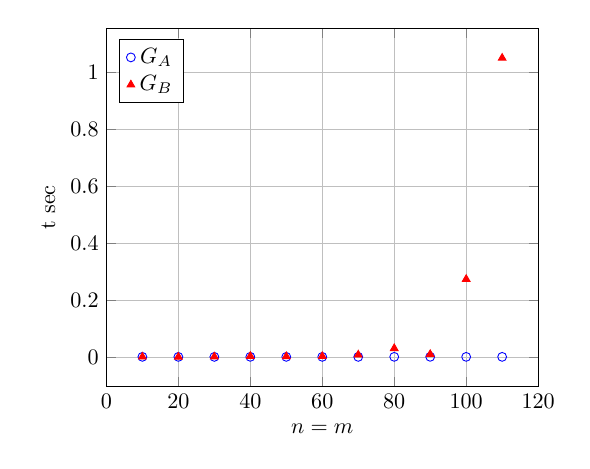
\begin{tikzpicture}[trim left=-1cm, scale=0.8]
	\begin{axis}[
	xlabel={$n=m$},
	ylabel=t sec,
	grid=both,
	legend pos=north west,
	extra tick style={grid=major, grid style={dotted, cyan}},
	extra x tick labels={},
	extra y tick style={grid=none}
	]
	\addplot[
	scatter,only marks,scatter src=explicit symbolic,
	scatter/classes={
		a={mark=o,blue},
		b={mark=triangle*,red}
	}
	]
	table[x=x,y=y,meta=label]{
		x    y    label
		10  0.000648975372314 a
		10  0.000707864761353 b
		20  0.000533103942871 a
		20  0.000607013702393 b
		30  0.000514030456543 a
		30  0.00131988525391 b
		40  0.000682830810547 a
		40  0.00321912765503 b
		50  0.000607013702393 a
		50  0.00205492973328 b
		60  0.000588893890381 a
		60  0.00267696380615 b
		70  0.000577926635742 a
		70  0.00788307189941 b
		80  0.000648975372314 a
		80  0.0305290222168 b
		90  0.000776052474976 a
		90  0.00965595245361 b
		100  0.000566959381104 a
		100  0.273800849915 b
		110  0.000571012496948 a
		110  1.05121898651 b
	};
	\legend{$G_A$, $G_B$}
	\end{axis}
	\end{tikzpicture}
	\caption{Graph $G_A$ versus $G_B$ for $n=m$}
	\label{fig:avb}
\end{figure}

\section{k-local Consistency Experimental Proof}
Here we provide experimental proof that using gauss elimination on versus off did indeed make a difference in times. We take graphs of two identical sizes, $n=300$ and $m=600$. For one system, we generated a uniquely satisfiable set of clauses without checking our stored version, which is the other. We convert both systems into graphs and find that one system is substantially slower than the other. We see that a system with a large  discrepancy in time gives rise to a drastically slower system. See Table \ref{table:tx}.

\begin{table}[h]
	\centering
	\begin{tabular}{l l l l}
		\toprule
		Instance 300:600 ($n:m$)& Gauss On & Gauss Off & Traces time  \\ 
		\midrule
		Random uniquely satisfiable system & 0.0078 & 0.0077 & 0.18 \\
		Likely $k$-locally consistent & 0.0074 & 0.0129 & 1.04 \\
		\bottomrule
	\end{tabular}
	\caption{Comparing two graphs. Both are $2n=m$ with $n=300$ and $m=600$}
	\label{table:tx}
	
\end{table}




%%!TEX root = ../thesis.tex
%*******************************************************************************
%****************************** Third Chapter **********************************
%*******************************************************************************
\chapter{Conclusion}

% **************************** Define Graphics Path **************************
\ifpdf
    \graphicspath{{Chapter3/Figs/Raster/}{Chapter3/Figs/PDF/}{Chapter3/Figs/}}
\else
    \graphicspath{{Chapter3/Figs/Vector/}{Chapter3/Figs/}}
\fi

In summary, we have presented and produced a family of graphs which execute slowly on the fast graph isomorphism solver Traces. We provided the capability to generate difficult graphs at random, satisfying  rigidity and resistance the vertex colour refinement algorithm underlying the solving program. We utilised a SAT solver, and implemented concepts from combinatorics, computational complexity and graph theory. Our package of graphs consistently took longer than three hours to execute for many instances. We successfully utilised Gaussian elimination and unique satisfiability of 3-XOR-Formulas as good guess of odd and $k$-locally consistent instances. Furthermore, we executed our searching algorithm for many thousands of iterations to incrementally increase the complexity of graphs. In addition, we provided experimental proof of the importance of $k$-local consistency when generating difficult instances. Including benchmark tests with existing graph families. 

Previously, the best known randomly generated graphs were those with differing edge probability. Here we provide open source code to randomly generate difficult graphs to further our understanding of the graph isomorphism problem.   

\section[Further Work]{Further Work}
During the time of this project, another analysis into benchmark graph isomorphism solvers was produced. The work in question is of Neuen and Schweitzer, which utilised similar ideas of multipedes to generate difficult graphs, however the approach differed in that shrunken multipedes were used, in contrast to our method of randomly generating such graphs from an 3-XOR-Formula \cite{neuen2017benchmark}. During the final stages of experiments, we selected a similar timeout value to this paper (three hours). We must clarify that this paper arose during our final stages, and influenced our work only by means of determining a timeout value. This was done to test our graph against the similar construction. Given that experiments were already underway, we point to this work to compare our own. Since different techniques were used to generate similar graphs. That is, using a form of reduction to make graphs more difficult. A point of departure would be to include the newly created package and test against this.

In this work, there is potential to find stronger and more difficult instances than the ones we have found. By using multiple experiments to build up a database of slow graphs, the ones we have provided in packages are assuredly not the slowest existing. To this end, a point of departure would be continuously run our searching algorithm, make improvements to the efficiency in locating and incorporate better techniques to find systems. The backbone of finding difficult graphs for the GI problem has been presented. With further work to this algorithm, we can undoubtedly come a step closer to understanding the graph isomorphism problem and its limits.


%\include{Chapter7/chapter7}



% ********************************** Back Matter *******************************
% Backmatter should be commented out, if you are using appendices after References
%\backmatter

% ********************************** Bibliography ******************************
\begin{spacing}{0.9}

% To use the conventional natbib style referencing
% Bibliography style previews: http://nodonn.tipido.net/bibstyle.php
% Reference styles: http://sites.stat.psu.edu/~surajit/present/bib.htm

\bibliographystyle{apalike}
%\bibliographystyle{unsrt} % Use for unsorted references  
%\bibliographystyle{plainnat} % use this to have URLs listed in References
\cleardoublepage
\bibliography{References/references} % Path to your References.bib file


% If you would like to use BibLaTeX for your references, pass `custombib' as
% an option in the document class. The location of 'reference.bib' should be
% specified in the preamble.tex file in the custombib section.
% Comment out the lines related to natbib above and uncomment the following line.

%\printbibliography[heading=bibintoc, title={References}]


\end{spacing}

% ********************************** Appendices ********************************

\begin{appendices} % Using appendices environment for more functunality

%!TEX root = ../thesis.tex
% ******************************* Thesis Appendix A ****************************
\chapter{How to install \LaTeX} 

\section*{Windows OS}

\subsection*{TeXLive package - full version}
\begin{enumerate}
\item	Download the TeXLive ISO (2.2GB) from\\
\href{https://www.tug.org/texlive/}{https://www.tug.org/texlive/}
\item	Download WinCDEmu (if you don't have a virtual drive) from \\
\href{http://wincdemu.sysprogs.org/download/}
{http://wincdemu.sysprogs.org/download/}
\item	To install Windows CD Emulator follow the instructions at\\
\href{http://wincdemu.sysprogs.org/tutorials/install/}
{http://wincdemu.sysprogs.org/tutorials/install/}
\item	Right click the iso and mount it using the WinCDEmu as shown in \\
\href{http://wincdemu.sysprogs.org/tutorials/mount/}{
http://wincdemu.sysprogs.org/tutorials/mount/}
\item	Open your virtual drive and run setup.pl
\end{enumerate}

or

\subsection*{Basic MikTeX - \TeX~ distribution}
\begin{enumerate}
\item	Download Basic-MiK\TeX (32bit or 64bit) from\\
\href{http://miktex.org/download}{http://miktex.org/download}
\item	Run the installer 
\item	To add a new package go to Start >> All Programs >> MikTex >> Maintenance (Admin) and choose Package Manager
\item	Select or search for packages to install
\end{enumerate}

\subsection*{TexStudio - \TeX~ editor}
\begin{enumerate}
\item	Download TexStudio from\\
\href{http://texstudio.sourceforge.net/\#downloads}
{http://texstudio.sourceforge.net/\#downloads} 
\item	Run the installer
\end{enumerate}

\section*{Mac OS X}
\subsection*{MacTeX - \TeX~ distribution}
\begin{enumerate}
\item	Download the file from\\
\href{https://www.tug.org/mactex/}{https://www.tug.org/mactex/}
\item	Extract and double click to run the installer. It does the entire configuration, sit back and relax.
\end{enumerate}

\subsection*{TexStudio - \TeX~ editor}
\begin{enumerate}
\item	Download TexStudio from\\
\href{http://texstudio.sourceforge.net/\#downloads}
{http://texstudio.sourceforge.net/\#downloads} 
\item	Extract and Start
\end{enumerate}


\section*{Unix/Linux}
\subsection*{TeXLive - \TeX~ distribution}
\subsubsection*{Getting the distribution:}
\begin{enumerate}
\item	TexLive can be downloaded from\\
\href{http://www.tug.org/texlive/acquire-netinstall.html}
{http://www.tug.org/texlive/acquire-netinstall.html}.
\item	TexLive is provided by most operating system you can use (rpm,apt-get or yum) to get TexLive distributions
\end{enumerate}

\subsubsection*{Installation}
\begin{enumerate}
\item	Mount the ISO file in the mnt directory
\begin{verbatim}
mount -t iso9660 -o ro,loop,noauto /your/texlive####.iso /mnt
\end{verbatim}

\item	Install wget on your OS (use rpm, apt-get or yum install)
\item	Run the installer script install-tl.
\begin{verbatim}
	cd /your/download/directory
	./install-tl
\end{verbatim}
\item	Enter command `i' for installation

\item	Post-Installation configuration:\\
\href{http://www.tug.org/texlive/doc/texlive-en/texlive-en.html\#x1-320003.4.1}
{http://www.tug.org/texlive/doc/texlive-en/texlive-en.html\#x1-320003.4.1} 
\item	Set the path for the directory of TexLive binaries in your .bashrc file
\end{enumerate}

\subsubsection*{For 32bit OS}
For Bourne-compatible shells such as bash, and using Intel x86 GNU/Linux and a default directory setup as an example, the file to edit might be \begin{verbatim}
edit $~/.bashrc file and add following lines
PATH=/usr/local/texlive/2011/bin/i386-linux:$PATH; 
export PATH 
MANPATH=/usr/local/texlive/2011/texmf/doc/man:$MANPATH;
export MANPATH 
INFOPATH=/usr/local/texlive/2011/texmf/doc/info:$INFOPATH;
export INFOPATH
\end{verbatim}
\subsubsection*{For 64bit OS}
\begin{verbatim}
edit $~/.bashrc file and add following lines
PATH=/usr/local/texlive/2011/bin/x86_64-linux:$PATH;
export PATH 
MANPATH=/usr/local/texlive/2011/texmf/doc/man:$MANPATH;
export MANPATH 
INFOPATH=/usr/local/texlive/2011/texmf/doc/info:$INFOPATH;
export INFOPATH

\end{verbatim}



%\subsection{Installing directly using Linux packages} 
\subsubsection*{Fedora/RedHat/CentOS:}
\begin{verbatim} 
sudo yum install texlive 
sudo yum install psutils 
\end{verbatim}


\subsubsection*{SUSE:}
\begin{verbatim}
sudo zypper install texlive
\end{verbatim}


\subsubsection*{Debian/Ubuntu:}
\begin{verbatim} 
sudo apt-get install texlive texlive-latex-extra 
sudo apt-get install psutils
\end{verbatim}

%!TEX root = ../thesis.tex
% ******************************* Thesis Appendix B ********************************

\chapter{Installing the CUED class file}

\LaTeX.cls files can be accessed system-wide when they are placed in the
<texmf>/tex/latex directory, where <texmf> is the root directory of the user’s \TeX installation. On systems that have a local texmf tree (<texmflocal>), which
may be named ``texmf-local'' or ``localtexmf'', it may be advisable to install packages in <texmflocal>, rather than <texmf> as the contents of the former, unlike that of the latter, are preserved after the \LaTeX system is reinstalled and/or upgraded.

It is recommended that the user create a subdirectory <texmf>/tex/latex/CUED for all CUED related \LaTeX class and package files. On some \LaTeX systems, the directory look-up tables will need to be refreshed after making additions or deletions to the system files. For \TeX Live systems this is accomplished via executing ``texhash'' as root. MIK\TeX users can run ``initexmf -u'' to accomplish the same thing.

Users not willing or able to install the files system-wide can install them in their personal directories, but will then have to provide the path (full or relative) in addition to the filename when referring to them in \LaTeX.



\end{appendices}

% *************************************** Index ********************************
\printthesisindex % If index is present

\end{document}
